% Nejprve uvedeme tridu dokumentu s volbami
\documentclass[czech,master]{diploma}
% Dalsi doplnujici baliky maker
\usepackage{amsmath}
\usepackage[autostyle=true,czech=quotes]{csquotes} % korektni sazba uvozovek, podpora pro balik biblatex
\usepackage[backend=biber, style=iso-numeric, alldates=iso]{biblatex} % bibliografie
\usepackage{dcolumn} % sloupce tabulky s ciselnymi hodnotami
\usepackage{subfig} % makra pro "podobrazky" a "podtabulky"
\usepackage[cpp]{diplomalst}
\usepackage{tikz}
\newcommand{\tikzxmark}{%
\tikz[scale=0.23] {
    \draw[line width=0.7,line cap=round] (0,0) to [bend left=6] (1,1);
    \draw[line width=0.7,line cap=round] (0.2,0.95) to [bend right=3] (0.8,0.05);
}}
\newcommand{\tikzcmark}{%
\tikz[scale=0.23] {
    \draw[line width=0.7,line cap=round] (0.25,0) to [bend left=10] (1,1);
    \draw[line width=0.8,line cap=round] (0,0.35) to [bend right=1] (0.23,0);
}}
\newcolumntype{C}[1]{>{\centering\let\newline\\\arraybackslash\hspace{0pt}}m{#1}}
% Zadame pozadovane vstupy pro generovani titulnich stran.
\ThesisAuthor{Bc. Lukáš Moravec}

\ThesisSupervisor{Ing. Radoslav Fasuga, Ph.D.}

\CzechThesisTitle{Principy automatizovaného obchodování na kryptoměnových burzách}

\EnglishThesisTitle{Principles of automated trading on cryptocurrency exchanges}

\SubmissionYear{2023}

\ThesisAssignmentFileName{assignment.pdf}

% Pokud nechceme nikomu dekovat makro zapoznamkujeme.
\Acknowledgement{Na tomto místě bych chtěl velice poděkovat všem, kteří mi pomohli při tvorbě této práce. Především patří můj vděk vedoucímu této diplomové práce, Ing. Radoslavovi Fasugovi, PhD., který věnoval mnoho času zodpovídáním otázek a konzultacemi.
Své díky chci vyjádřit také mému kolegovi, Bc. Josefu Žáčkovi, jenž vytvořil systém pro stahování historických dat pro kryptobota. Poděkování patří taktéž mé přítelkyni a mé rodině za trpělivost a podporu.}

\CzechAbstract{Diplomová práce cílí na vytvoření kryptoměnového bota. Popisuje kryptoměny a zmiňuje jakým způsobem se aktuálně kryptoměny obchodují.
Součástí práce je krátký úvod do technické analýzy včetně popisu několika grafových vzorů a technických indikátorů jakožto možný způsob pro analýzu kryptoměnových
párů a automatizování obchodování.
Dále lze v práci přečíst srovnání několika vybraných existujích kryptobotů a legislativní rámec týkající se kryptoměn.
V praktické části je popsán implementovaný kryptobot, který na základě vytvořených obchodních příkazů uskutečňuje reálné obchody na burze. Výsledný kryptobot byl napsán v jazyce Python
a pro persistenci dat využívá SŘBD MySQL.}

\CzechKeywords{kryptoměny; kopce a doliny; burza; technická analýza; Python; kryptobot}

\EnglishAbstract{The thesis aims to create a cryptocurrency trading bot.
It describes cryptocurrencies and mentions how cryptocurrencies are currently traded.
The thesis includes a brief introduction to technical analysis, including a description of several chart patterns and technical indicators as a possible way to analyze
cryptocurrency pairs and automate trading.
In addition, the thesis compares several selected existing crypto-bots and the legislative framework regarding cryptocurrencies.
The practical part describes the implemented crypto-bot, which executes real trades on the exchange based on created trading orders.
The resulting crypto-bot was written in Python and uses MySQL as a database management system for data persistence.
}

\EnglishKeywords{cryptocurrency; peak and valley, exchange; technical analysis, Python; cryptobot}

\AddAcronym{GTC}{Good-Till-Cancel}
\AddAcronym{FOK}{Fill-Or-Kill}
\AddAcronym{IOC}{Immediate-Or-Cancel}
\AddAcronym{OCO}{One-Cancels-the-Other}
\AddAcronym{PoS}{Proof-of-Stake}
\AddAcronym{PoA}{Proof-of-Authority}
\AddAcronym{PoW}{Proof-of-Work}
\AddAcronym{DPoS}{Delegated Proof-of-Stake}
\AddAcronym{DeFi}{Decentralized Finance}
\AddAcronym{MiCA}{Markets in Crypto-Assets}
% \AddAcronym{HTML}{Hyper Text Markup Language}
% \AddAcronym{TUG}{\TeX{} Users Group}

\addbibresource{bibliography.bib}

% Novy druh tabulkoveho sloupce, ve kterem jsou cisla zarovnana podle desetinne carky
\newcolumntype{d}[1]{D{,}{,}{#1}}


% Zacatek dokumentu
\begin{document}

% Nechame vysazet titulni strany.
\MakeTitlePages

% Jsou v praci obrazky? Pokud ano vysazime jejich seznam a odstrankujeme.
% Pokud ne smazeme nasledujici dve makra.
\listoffigures
\clearpage

% Jsou v praci tabulky? Pokud ano vysazime jejich seznam a odstrankujeme.
% Pokud ne smazeme nasledujici dve makra.
\listoftables
\clearpage

% A nasleduje text zaverecne prace.
\chapter{Úvod}
\label{sec:Introduction}
Kryptoměnové trhy, obchodování a celková budoucnost tohoto fenoménu je zajímavým tématem dnešní doby. Vysoká volatilita, jakožto jedna z hlavních charakteristik tohoto trhu, s sebou přináší
možnost interesantních strategií obchodování. Tato práce je zaměřena na nalezení vhodných příležitostí obchodování kryptoměnových párů na světových burzách. Hlavním cílem
je vytvořit nástroj pro automatizované provádění technické analýzy a obchodování kryptoměn.

Teoretická část práce, která je zároveň první částí, se zaměřuje na obecný popis kryptoměn, co to je kryptoměna, blockchain a jakými způsoby probíhá ověřování validní transakce. Dále jsou
přiblíženy kryptoměnové burzy, jejich historie a poskytované funkce. S burzami se pojí i obchodní příkazy. Rozdíly mezi jednotlivými obchodními příkazy a způsob, jak jsou vykonávány je
součástí první části práce.

Druhá kapitola se zabývá technickou analýzou, jež slouží jako základ pro automatizované obchodování kryptobota. Je zde uvedena historie technické analýzy a hlavní principy
na kterých je postavena. Důležitou součástí této kapitoly jsou grafové vzory a technické indikátory. Pro názornost je součástí každého vzoru i indikátoru vizualizace.

Následující, třetí, kapitola analyzuje existující kryptoboty a jejich funkce. Vysvětluje, na jakých hlavních bodech kryptoboti staví respektive, jak lze kryptoboty rozdělit do několika
kategorií. Shrnují se zde výhody a nevýhody oproti tradičnímu obchodování.

Předposlední kapitola je věnována legislativě. Popisuje se převážně český legislativní rámec kryptoměn, jejich obchodování a danění. Důležitou částí je však taky popis chystané evropské
regulace MiCA. Je zde uvedeno, jak MiCA kategorizuje kryptoaktiva a jednotlivá pravidla pro vydávání a zacházení s nimi.

Finální kapitola se zabývá praktickou implementační částí. Popsán je hlavní princip kryptobota, využité metody technické analýzy a scénáře obchodování. Čtenáři je blíže přiblíženo, jak
kryptobot vybírá vhodné páry k obchodování. Součástí je i popis jednotlivých případů opakování obchodních příkazů a skutečné provedení. V rámci kapitoly je uvedeno, jak probíhá komunikace
s burzou Binance. Poslední částí této kapitoly je shrnutí vykonaných obchodů a výdělečnosti kryptobota. Dále je popsáno, jak lze bota rozšířit, jaké funkce lze přidat tak, aby se stal ještě
robustnějším nástrojem pro ziskové obchodování.

\endinput
\chapter{Kryptoměny a obchodování na burzách}
\label{sec:CryptoAndTrading}

Fenomén Bitcoinu, který jako první odstartoval kryptoměnový boom, způsobil várku mnoha nových
kryptoměn, založených buďto na podobných principech a technologiích, nebo s novými inovativními myšlenkami.
Spolu s kryptoměnami přišlo spoustu nového názvosloví, byly nimi inspirovány NFT\footnote{Non-fungible tokens} a vzniklo
nové odvětví digitálních financí, označováno jako DeFi (decentralizované finance).
Tato kapitola postupně popíše co to jsou kryptoměny, s využitím jakých technologiích fungují, jak jsou ověřovány
a obchodovány na burzách.


\section{Coiny, chytré kontrakty a tokeny}
\label{sec:CoinsTokensSmartContracts}
Často se lze setkat s pojmy \enquote{token} nebo \enquote{coin}. Obojí se označuje za kryptoměnu a mnohdy se zaměňují
za jednu a tu stejnou věc. Jak token, tak i coin žijí na blockchainu.
Koncept blockchainu je vysvětlen v následují sekci. Co je to vlastně token nebo coin? Jak již bylo zmíněno, obojí využívá
blockchain, avšak hlavní rozdíl spočívá v tom, co reprezentují. Coin označuje kryptoměnu používanou k uchovávání
nebo směny hodnoty. Jako příklad je možné považovat například známí Bitcoin. Token slouží k digitální reprezentaci
aktiva, které se dá směnit pomocí blockchainu. Token může reprezentovat nejen fyzickou věc, jako například zlato, ale i
duševní vlastnictví. Důvodem, proč se tyto pojmy často zaměňují je, že token může reprezentovat \emph{coin} na jiném blockchainu.

Myšlenka chytrých kontraktů poprvé zazněla už v roce 1997. Chytrý kontrakt měl odstranit potřebu důvěry třetí strany při
jednání nebo \enquote{sjednání smlouvy} s někým druhým. Typickým problémem je skupinové financování (crowdfunding). Prostřednictvím
nějakého poskytovala si kdokoli může vytvořit svůj projekt a požádat veřejnost o pomoc k dosažení finančního cíle. Jestliže se najde dostatek
jednotlivců, ochotných přispět na daný projekt a vysbírá se dostatek finančních prostředků, peníze poputují k zadavateli a ten s touto podporou
svůj projekt uskuteční. V opačném případě, kdy se nepodaří dosáhnout minimální finanční podpory, se peníze musí vrátit zpět všem investorům.

Chytré kontrakty na blockchainu jsou v podstatě malé programy, napsány ve speciálním programovacím jazyce, plnící přesně tuto funkci prostředníka.
Jakmile je jednou chytrý kontrakt publikován, je neměnný a distribuovaný sítí. Skutečnost, že je kontrakt distribuovaný
taktéž znamená, že jeho platnost je ověřována všemi členy na dané síti.
Jelikož se jedná o program, jakmile je dosaženo konkrétního cíle, okamžitě se vykoná finální akce. Z předchozího příkladu veřejného
financování, by se dal chytrý kontrakt naprogramovat tak, aby držel všechny přijaté platby dokud není dosaženo minimální částky.
Tento proces je však naprosto transparentní a automatizovaný.


\section{Ověřování transakcí}
\label{sec:BlockchainSecurity}
Hlavní motivace kryptoměn je možnost platit pomocí Internetu bez toho, aniž by platba byla závislá na centrální autoritě, která by měla
být ověřený a důvěryhodný prostředník. Může se však stát, že i tato centrální autorita nesplní své závazky vůči oběma stranám.

V roce 2008 zveřejnil neznámý autor, či skupina autorů, pod názvem Satoshi Nakamoto kryptoměnu Bitcoin a s ní i systém bezpečného
ověřování plateb bez nutnosti centrální autority. Dva nejdůležitější faktory tohoto zabezpečení spočívají v počítačové kryptografii
a distribuci dat. Co to tedy vlastně je blockchain a jak funguje je vysvětleno na následujícím příkladu.

Nechť existují 4 osoby, Alice, Bob, Ctirad a David. Tyto osoby, aby si nemusely pořád předávat peníze, si vedou jednotnou digitální účetní knihu,
pro kohokoli z této čtveřice dostupnou. Pokud má Alice zaplatit Bobovi 20 Kč, zapíšou si údaj o této transakci do účetní knihy. Vždy na
konci měsíce se všichni 4 sejdou a opravdové peníze mezi sebou vymění. V tento moment se naráží na první závažnou chybu v tomto systému.
Účetní kniha je veřejně dostupná a každý do ní může zapsat jakoukoli transakci. Nic nebrání tomu, aby si David do účetní knihy zapsal, že
mu mají všichni zaplatit 10 Kč. Tyto záznamy nejdou ověřit a jsou nedůvěryhodné. Řešení této situace spočívá v použití kryptografie,
konkrétně digitálních podpisů. Ke každému záznamu bude muset být přiložen podpis o tom, že osoba předávající peníze tuto transakci předem
viděla a schválila. Digitální podpisy se zakládají na dvojici privátního a veřejného klíče. Je nutné privátní klíč udržet v tajnosti,
pouze pro sebe. Samotný podpis můžeme chápat jako funkci, která na základě vstupní zprávy a privátního klíče, vygeneruje číslo o pevné velikosti,
nejčastěji 256 bitů. Výhodou digitálního podpisu je právě to, že je závislý na vstupu. Pokud se jakkoli změní, je vygenerovaný podpis
naprosto odlišný. Aby šlo ověřit, že podpis je skutečně platně podepsán osobou vlastnící privátní klíč, existuje druhá funkce, schopná
toto ověření provést. Ověření probíhá na základě původní vstupní zprávy, podpisu a veřejného klíče. Výstupem této funkce je pravdivostní
hodnota říkající, zda-li podpis dané zprávy byl vygenerován za použití přidruženého privátního klíče. Tímto je skoro vyřešen problém ověření
pravdivosti transakce v účetní knize. Aby se předešlo falšování pouhým kopírováním předešlého už podepsaného záznamu, přiřazuje se záznamu
transakce taktéž její číselné pořadí.

Nyní nastává další problém. Co se stane, pokud Ctirad nasbírá na účetní knize obrovské dluhy a na konci měsíce se prostě neukáže a uteče?
Pořád je nutná určitá část důvěry. Řešení je jednoduché. Je potřeba mít na úplném začátku knihy záznamy o tom, že všichni 4 dostanou
určitou část peněz, kterou nejdříve vloží do tajného trezoru. Dále už jen stačí jednoduše nedovolit nikomu přidávat
nový záznam o transakci, pokud na to nemá prostředky.

Zbývá poslední překážka a to správa o samotnou digitální účetní knihu. Ta musí někde existovat a musí být všem poskytovaná. To ale pořád
implikuje

 centrální umístění. Ke zbavení se této obtíže a úplné decentralizace, dostane každý účastník svou kopii účetní knihy. V digitálním světě
to znamená, že
každý účastník bude mít nějaké zařízení, na kterém bude mít kompletní kopii digitální účetní knihy a bude zveřejněna všem ostatním účastníkům,
na jakékoliv síti. Nyní, když všichni mají svou vlastní kopii, musí si umět navzájem vyměnovat informace o proběhlých transakcích a to formou
zpráv posílaných po síti. Aby měli všichni účastníci jistotu, že příjmají stejné zprávy a ve stejném pořadí jako ostatní, vyvstává finální
ověřovací krok. Účetní kniha se rozdělí do jednotlivých bloků, obsahující \emph{N} transakcí. Na závěr každého bloku se přidá speciální
číslo --- \emph{nonce}. Přidání \emph{nonce} se řídí určitým pravidlem, které říká, že prvních \emph{M} čísel hashe bloku budou samé nuly.
Hash bloku je vypočten kryptografickou hashovací funkcí\footnote{Nejčastěji se jedná o funkci SHA-256} ze všech záznamu na zapsaných na bloku
a přidaného nonce. Kvůli vlastnostem hashovacích funkcí, nelze nonce nějak jednoduše vypočítat, ale je nutné jej uhádnout brutální výpočetní silou.
Jakmile někdo z účastníků na této síti transakcí přijde na nonce nějakého bloku, rozešle tento blok s transakcemi a přidaným nonce.
Ostatní účastnici ověří platnost bloku a uloží si ho. Navíc, aby nešlo pořadí bloků zaměňovat, každý nový blok musí v pomyslné hlavičce
obsahovat hash předchozího bloku. Tímto dochází ke zřetězení bloků (odtud název blockchain).

Takto funguje princip ověřování transakcí na základě tzv. proof-of-work. Věří se vždy tomu blockchainu, do kterého bylo dáno nejvíce
výpočetní síly, tzn. tomu nejdelšímu řetězu bloků. V reálném světě účastníkem v nějaké kryptoměnové síti jsou počítače, zvané nody.
Na nodech se ukládá blockchain a jak již avizováno, věří se vždy tomu nejdelšímu retezu bloků. Svůj vlastní node si může u sebe doma spustit
téměř kdokoli. Pravidla pro přidávání nonce se mohou lišit v závislosti na kryptoměně.

Zde je také vhodné zodpovědět otázku, jak vlastně kryptoměna vzniká. V uvedené analogii si 4 osoby vložili peníze do společného banku.
Ve světě blockchainu je to takzvaným Genesis blokem (někdy také nazýván \enquote{Block 0}). Jako Genesis blok se označuje úplně první
vytěžený blok, na který všechny ostatní bloky v blockchainu navazují. Těžbou bloků se zde myslí právě nalezení nonce, který se přidává do patičky
bloku. Těžař jako odměnu za vynaložené usílí a výpočetní výkonu dostává kryptoměnu ve formě speciální transakce přidané na konci vytěženého bloku.
Maximální velikost odměny je specifikována protokolem, kterým těžba probíhá a těžaři respektují.

\subsection{Alternativní ověřování --- proof-of-stake}
\label{proof-of-stake-subsection}
Ověřování na základě proof-of-work má 2 zásadní nevýhody. První z nich je ta, že odměny na základě těžby bloků nepřímo podněcují centralizaci.
Jelikož vyšší výpočetní výkon znamená vyšší šanci na úspěch při těžbě bloků, stává se, že těžaři se spojují do tzv. \enquote{mining pools}.
V těchto poolech je odměna za vytěžení bloku rozdělena mezi jednotlivé účastníky. Jestliže však mining pool naroste do rozměru, kdy by tvořil
alespoň 51 \% výpočetního výkonu kryptoměnové sítě, teoreticky bude tento pool schopen tvořit nové bloky s falešnými transakcemi. Tato situace
bývá označována jako \enquote{51\% útok} a při jeho úspěšném provedení dochází ke kolapsu kryptoměny. Nicméně k jeho úspěšnému dosažení je potřeba velké množství prostředků.

Druhým problémem proof-of-work je vysoká energetická náročnost. V době psaní této práce se odhaduje roční energetická náročnost těžby pouze Bitcoinu
na 88,5 TWh \cite{crypto:energy-consumption-bitcon}. Pro srovnání, celá Česká republika za rok 2021 spotřebovala okolo 466 TWh \cite{crypto:energy-consumption-czechia}.
Tato spotřeba zatěžuje jak rozvodné elektrické sítě tak i těžaře.

Převážně z důvodu velké spotřeby elektřiny v roce 2012 byl představen alternativní přístup k ověřování transakcí, označovaný jako proof-of-stake (dále jen PoS).
PoS upravuje tradiční terminologii, těžaře nahrazuje \emph{validátory} a namísto \enquote{těžby} jsou bloky \emph{\enquote{raženy}}. PoS je 
postaven na konsenzu mezi účastníky v síti. Bloky jsou ověřovány náhodně vybranými validátory, kteří jednotlivé transakce ověří a označí za platné.
Tento validovaný blok je následně přidán do blockchainu. Aby se z účastníka stal validátor, stačí se jednoduše do sítě nabídnout a vložit určitou
\enquote{sázku} (stake). Výše této sázky ovlivňuje pravděpodobnost výběru při selekci validátorů k ověření bloku. Pokud by validátor označil
blok obsahující falešné transakce jako platný, je mu část nebo celá vložená sázka odebrána. Tento postih má být motivací, aby validátoři doopravdy
odváděli svou práci správně. Kriticky důležitý krok při ověřování je výběr validátorů. I u této metody ověřování existuje možnost 51\% útoku,
avšak k dosažení je nutné nabídnout alespoň o něco víc než polovinu tržní kapitalizace kryptoměny, čehož není jednoduché dosáhnout.
Na proof-of-stake již funguje celá řada kryptoměn, mezi největší se řadí například Ethereum, BNB a Cardano.

Nově vznikají další metody jak dosáhnout společného konsenzu na blockchainu. Jedním z těchto nových způsobů je proof-of-authority (PoA). I tato
metoda využívá validátory, nicméně tito validátoři ručí svou vlastní reputací a důvěryhodností. Validátoři jsou předem vybráni autoritou a mají
za úkol ověřovat a přidávat nové bloky do blockchainu. Tento algoritmus pro dosažení konsenzu je vhodnější spíše pro soukromé blockchainové sítě,
jelikož v něm pracuje omezený počet validátorů a neumožňuje velkou decentralizaci.

Dalším algoritmem je delegovaný proof-of-stake (DPoS). Omezený počet validátorů bloků je volen účastníky sítě. Váha volebního hlasu
je určena množstvím kryptoměny, kterou uživatel na blockchainu disponuje. Zvoleným validátorům se taktéž přezdívá delegáti. Zvolený delegát má pak
na starosti validaci transakcí a přidávání nových bloků do blockchainu. Aby se více pojistila důvěryhodnost delegátů, musí se zaručit množstvím
své vlastní kryptoměny, o kterou, v případě pochybení, přijdou.


\section{Kryptoměnové burzy}
\label{sec:Exchanges}
Dříve, když byly kryptoměny na svém počátku neexistovalo mnoho možností jak tuto digitální měnu získat. Volby byly buďto měnu vytěžit, nebo
si na internetovém fóru dohodnout P2P obchod. Jedním z takových internetových fór byl Bitcointalk, který založil sám 123 Satoshi Nakamoto právě proto,
aby se něm vedla diskuze ohledně Bitcoinu. P2P obchody mohly být riskantní, jelikož obchod byl domluvený s cizincem přes internetové fóru, kterému
se uživatel rozhodl důvěřovat. V roce 2010 se začali objevovat první směnárny, největší z nich se stala Mt. Gox. Tato směnárna se starala o více jak polovinu
všech světových bitcoinových transakcí, avšak kvůli častým bezpečnostním průlomům a vykrádání musela v roce 2014 ukončit činnost.

V současné době existuje větší rozmanitost kryptoměnových burz. Tyto nové burzy už neplní pouze funkci směnárny, ale skutečně nabízejí možnosti
kryptoměny obchodovat, podobně jako například na akciovém trhu. Jako další metodou investice lze také využít \emph{staking}. Na první pohled se staking
může zdát jako jakýsi ekvivalent termínovaného vkladu v té podobě, že člověk zastaví svá aktvita na nějakou určitou dobu. Na konci tohoto období dostane
odměnu v podobně coinů, nebo v případě termínovaných vkladů, peněz. V realitě se ale termínovaný vklad od stakingu ve své podstatě liší. U termínovaného
vkladu dává zákazník bance určitou částku peněz k obchodu a investicím. Banka jako odměnu vyplatí část peněz zpět ve formě předem domluveného úroku.
Staking je aktivní podílení se na ověřování transakcí na \emph{proof-of-stake} blockchainu popsané v předchozí části
\ref{proof-of-stake-subsection}. Tak jako u proof-of-work existují mining pooly, tak i u proof-of-stake vznikají staking pooly, ve kterých uživatelé
blockchainu společně vloží své coiny a stanou se validátorem. Odměnu si pak rozdělí podle vložených coinů. Burzy v tomto ohledu velice zjednodušují
celý princip stakingu, jelikož tyto pooly řídí na pozadí a uživatel si pouze vybírá, se kterým coinem chce stakovat a na jak dlouhou dobu. Navíc k tomu
burza může uživateli poskytnout lepší odhady o získané odměně, risku apod.

K vizualizaci trendů a aktuální tržní ceny využívají burzy grafické znázornění ve formě grafů. Typicky poskytují 3 typy grafů --- spojnicový, sloupcový a svíčkový.
Investoři si samozřejmě mohou vybrat nejvíce vyhovující jejich gestu. Rozdíly mezi grafy nejsou pouze vizuální, ale liší se také množství informací, jaké z nich lze vyčíst.
Obvykle se v těchto grafech zobrazují ceny kryptoměn za určité časové okno (1 minuta, 1 hodina, \ldots). Oproti spojnicovému grafu dokáže sloupcový a svíčkový
zobrazit otevírací (open), nejvyšší (high), nejnižší (low) a závěrečnou (close) cenu kryptoměny v daném okně.

\subsection{Obchodování kryptoměn}
Obchodování kryptoměnových párů má vesměs stejný princip jako forexový trh. Obchodník směňuje jednu měnu za druhou a snaží se vydělat na rozdílu jejich tržních cen.
Jednotlivé měny v páru jsou označovány jako podkladová (angl. base) a kotovaná (angl. quote) měna. Zapisují se ve formátu {BBB/QQQ}, tedy například při zápise
EUR/USD je euro podkladová měna a dolar kotovaná. Podkladová měna je vždy rovna 1, tzn. pokud je kurz EUR/USD roven $1,2$ znamená to, že za nákup 1 eura
obchodník zaplatí $1,2$ dolaru. Vždy tedy platí:
\begin{itemize}
    \item během nakupování se platí kotovanou měnou za měnu podkladovou,
    \item při prodeji se prodává podkladová měna a získává měna kotovaná.
\end{itemize}
Dále v této práci mohou být tyto názvy použity i v jejich anglickém překladu.

\begin{figure}[ht]
    \centering
    \subfloat[\centering Spojnicový graf]{{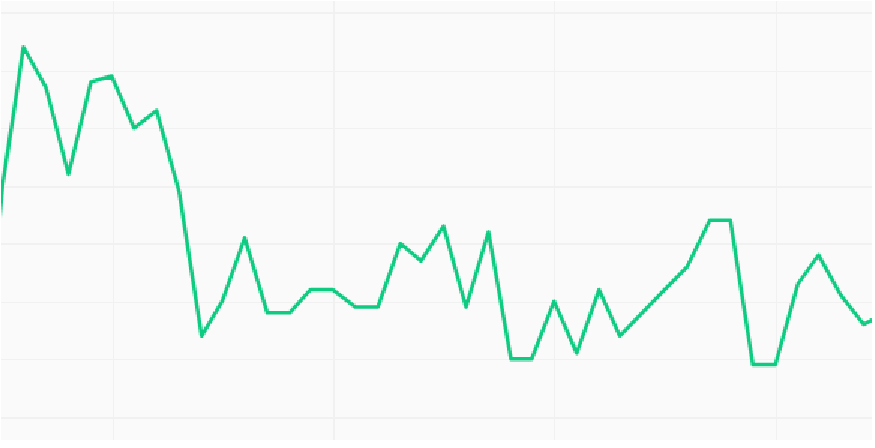
\includegraphics[width=0.45\textwidth]{Figures/linechart.pdf}}}
    \qquad
    \subfloat[\centering Sloupcový graf]{{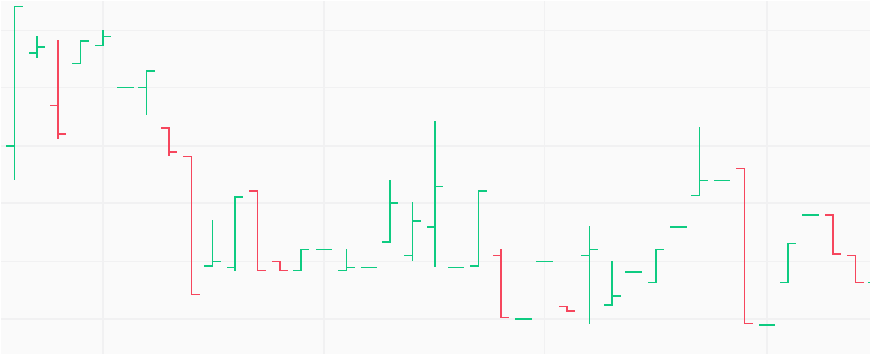
\includegraphics[width=0.45\textwidth]{Figures/barchart.pdf}}}

    \subfloat[\centering Svíčkový graf]{{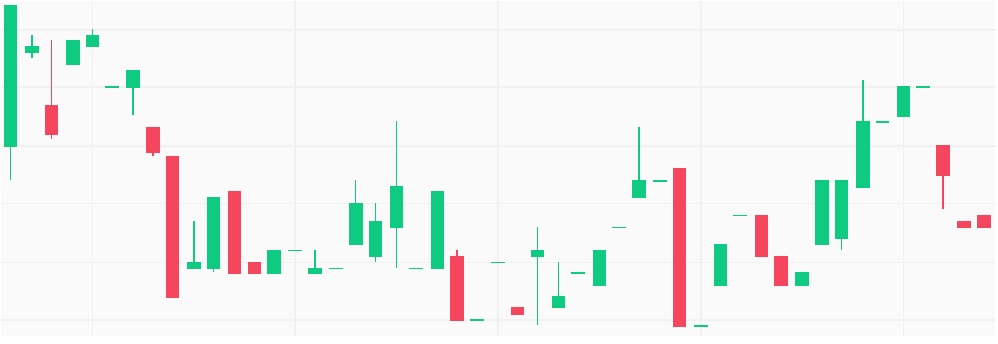
\includegraphics[width=0.45\textwidth]{Figures/candlestickchart.pdf}}\label{subfig:candlestickchart}}
    \qquad
    \subfloat[\centering Svíčka]{{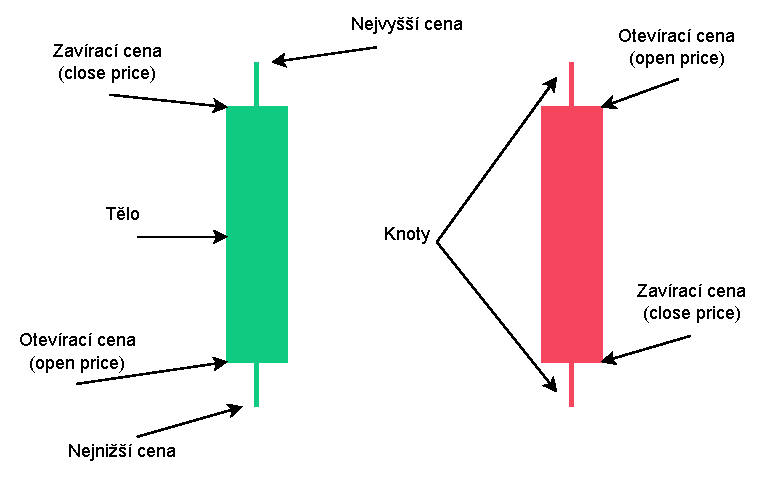
\includegraphics[width=0.45\textwidth]{Figures/candle.pdf}}}

    \caption{Používané grafy a popis svíčky}
    \label{fig:most-used-charts}
\end{figure}


\subsection{Obchodní příkazy}
\label{subsec:market-trade-orders}
Automatizovanou burzu tvoří 2 základní pilíře obchodování. První z nich je obchodní \enquote{kniha} neboli \emph{order book}. Order book není v podstatě nic
jiného než jen seznam nákupních a prodejních příkazů nějakého aktiva (například kryptoměny). Tento seznam bývá zorganizovaný podle ceny v těchto příkazech.
Druhý pilíř je systém, který se stará o párování těchto prodejních a nákupních příkazů, označovaný jako \emph{matching engine}. Ten tedy spáruje obchodní příkazy
a provede mezi nimi obchod. Ať už jeden, nebo i vícero obchodů.

Moderní burzy poskytují 2 odlišné typy příkazů. Příkaz \textsc{market} jde ihned na order book a otevírá pozici na momentální tržní ceně aktiva. Pokud uživatel
pošle/zadá tento příkaz, je okamžitě vykonán a to jak v prodejní tak i případné nákupní podobě. Druhým příkazem, který už nabízí jakousi možnost automatizace
je \textsc{limit}.
Limit se zadává s hraniční cenou, za kterou je uživatel aktivum ochotný nakoupit nebo prodat. Matching engine se snaží spárovat limit tak, aby byla splněna podmínka
hraniční ceny se spárovaným příkazem. Tato situace je jak pro prodej tak i pro nákup zachycena na obrázcích \ref{subfig:limit-buy} a \ref{subfig:limit-sell}.

V kombinaci s limit příkazem lze využít další 2 možné příkazy, označované jako \textsc{stop-limit} a \textsc{trailing stop-limit}. Oba přidávají další možnosti,
jak obchodování automatizovat. Stop-limit (\ref{subfig:stop-limit}) příkaz umožňuje přidat další cenový parametr, označovaný jako stop-cena neboli taky aktivační cena.
Tato stop-cena se chová jako zábrana, jelikož nepustí příkaz na order book, dokud není překročena. Například, pokud je aktuální tržní cena aktiva na 100\texteuro, uživatel zadává na burzu stop-limit příkaz k
prodeji se stop-cenou nastavenou na 110\texteuro a limit cenou na 95\texteuro. I přestože je splněna podmínka pro prodej k je tržní cena vyšší než limitní
a mohlo by dojít k zobchodování matching engine nemůže příkaz zobchodovat, jelikož stop-cena drží příkaz mimo order book. V momentě, kdy tržní cena vyšplhá na
alespoň 110\texteuro, je příkaz puštěn na order book a matching engine může vykonat obchod.
Trailing stop-limit (\ref{subfig:trailing-delta}) bere tuto myšlenku ještě o krok dále a umožňuje lepší zachycení trendu tržní ceny.
Tento příkaz počítá procentuální změnu ceny od lokálního
extrému (minimum pro nákup, maximum pro prodej), jakmile rozdíl ceny překročí uživatelem nastavenou hranici, je příkaz zapsán do order booku. Trailing-stop-limit
může taktéž mít nastavenou stop-cenu, tedy musí být splněna podmínka jak stop-ceny tak i procentuálního rozdílu.
Správné nastavení těchto parametrů je důležitým aspektem pro úspěšné zobchodování zadávaného příkazu. Například, pokud při zadávání trailing stop-limit příkazu
je zadaný rozdíl od extrému příliš malý, může být příkaz zobchodován dřív než by to doopravdy bylo výhodné nebo chtěné. Naopak, jestliže by rozdíl byl příliš velký
nemusí k zobchodování dojít vůbec a příkaz bude na burze nebude nic dělat.


\begin{figure}[ht]
    \centering
    \subfloat[\centering Oblast pro nákup]{{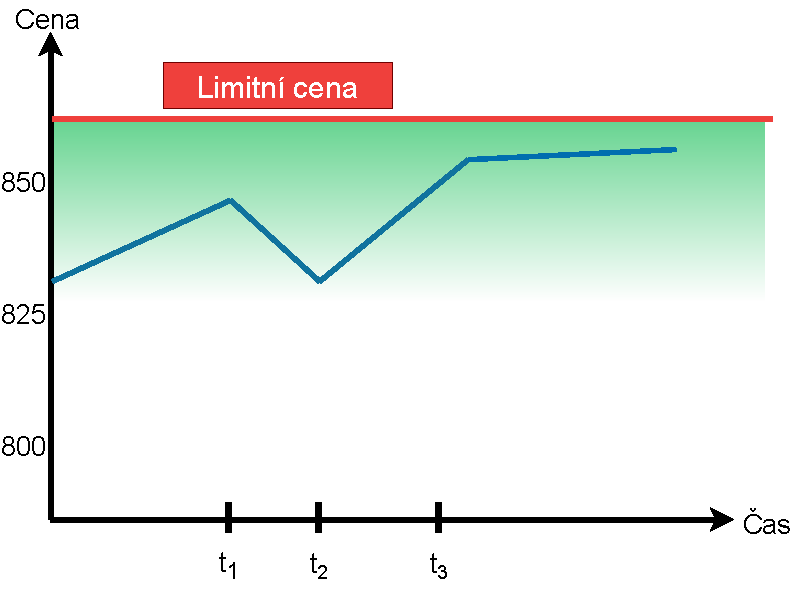
\includegraphics[width=0.45\textwidth]{Figures/limit-chart-buy.pdf}}\label{subfig:limit-buy}}
    \qquad
    \subfloat[\centering Oblast pro prodej]{{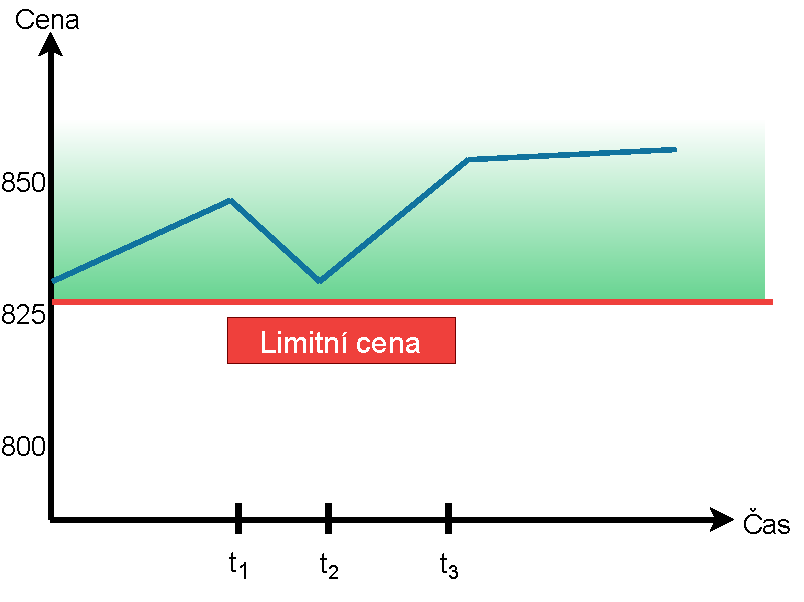
\includegraphics[width=0.45\textwidth]{Figures/limit-chart-sell.pdf}}\label{subfig:limit-sell}}

    \subfloat[\centering \textsc{stop limit} nákup]{{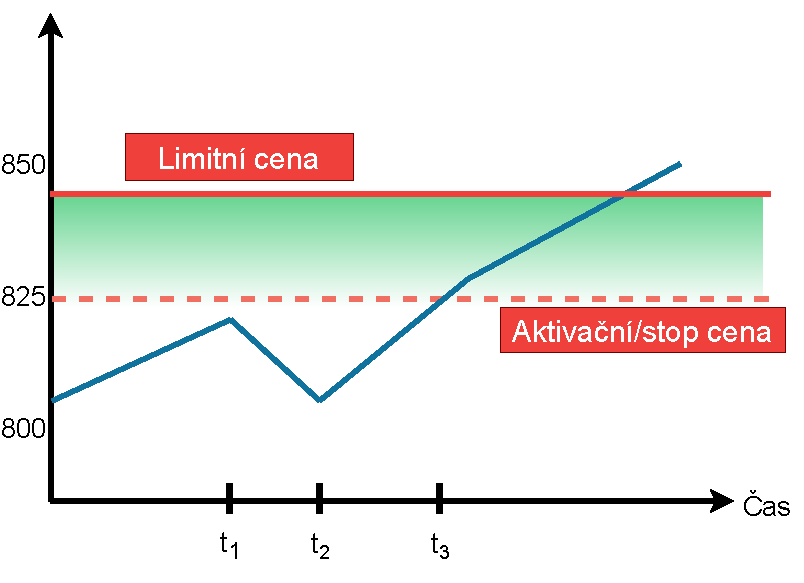
\includegraphics[width=0.45\textwidth]{Figures/stop-limit.pdf}}\label{subfig:stop-limit}}
    \qquad
    \subfloat[\centering Trailing]{{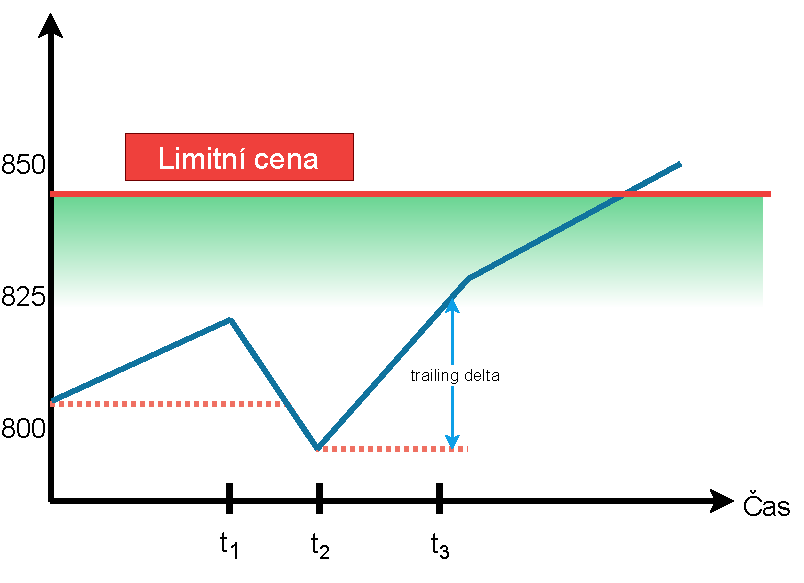
\includegraphics[width=0.45\textwidth]{Figures/trailing-delta.pdf}}\label{subfig:trailing-delta}}
    \caption{Příkaz limit s hraniční cenou}
    \label{fig:limit-orders}
\end{figure}


% Scalping, swinging, day trading, HODL
\subsection{Strategie obchodování}
Způsobů, jakým lze obchodovat na burzách může být až nekonečně mnoho. Jelikož se kryptoměnové burzy velice podobají forexovým, mohou se uplatnit podobné
obchodní strategie. Některé strategie mohou fungovat lépe nebo hůře v závislosti na obchodovaném aktivu.
Každý uživatel si může zvolit svou vlastní strategii, tak aby mu vyhovovala a pár z nich popisuje tato podsekce.

\subsubsection{Day trading}
Denní obchodování nebo-li \emph{day trading} se zaměřuje, jak název napovídá, na obchody netrvající déle než den. Tito obchodníci se snaží najít co nejvýhodnější
bod pro nákup a prodej aktiva v rámci jednoho dne a snaží se držet svou pozici nejdelší rozumnou dobu, aby mohli následně svou pozici uzavřít (prodat) se ziskem.
Těchto pozic neotevírají hodně, spíš jen pár za celý obchodní den.

\subsubsection{Scalping}
\label{subsubsec:scalping}
Tito obchodníci, nazývání \enquote{skalpeři} se snaží vydělat na mnoha malých, ale profitabilních obchodech. Pozice drží otevřené krátkou dobu, většinou pár minut
s nejdelší možnou dobou až pár hodin. Často využívají i \emph{pákového efektu}\footnote{Pákový efekt umožňuje traderovi otevřít pozici s násobenou kupní silou
    a tím i možností jak vyššího zisku, tak i případné ztráty.}. Hlavní podstata této strategie je dosáhnou zisku i z malých změn tržní hodnoty aktiva.
K rozhodování o otevření pozic se opírají o \emph{technickou analýzu}, která bude detailněji popsána v kapitole \ref{chap:TechnicalAnalysis}.

\subsubsection{Swing trading}
Swing tradeři sporadicky otevírají a zavírají pozice na trhu, přičemž své pozice drží i v období několika dnů, nebo týdnů. Čekají na větší cenové
výkyvy (doslova zhoupnutí ceny, odtud název swing trading) a tomu odpovídá i delší doba trvání obchodu. Využívají technickou analýzu ale i fundament
daného aktiva a snaží se odhadnout dlouhodobější trendy.

\subsubsection{Buy-and-hold}
Tato poslední metoda obchodování je čistě dlouhodobá a jedná se pouze o nákupy aktiv. Převážně oblíbená v krypto komunitě dostala tato strategie přezdívku HODL.
Vyhýbáním prodeje se investoři snaží mířit na výhledový zisk z držení. Podle motivace a filozofie HODLerů je vždy skvělá příležitost nakoupit kryptoměnu a za
žádných okolností neprodávat, ale držet své coiny u sebe.

\endinput
\chapter{Technická analýza}
\label{chap:TechnicalAnalysis}
Dělat informovaná rozhodnutí je podstata každého obchodníka. V akciových trzích se významně používá fundamentální analýza používaná pro budoucí odhad
chování trendu trhu. Fundament se zabývá vnitřní hodnotou trhu, která je spjatá s obchodními výsledky podniků obchodovaných na burze. Tyto dvě faktory,
tedy dlouhodobé obchodní výsledky podniků často korelují právě s hodnotou akcií. Vnitřní hodnota trhu je pak odhadována za momentální hodnotou jmění
těchto firem. Odhady lze dělat z veřejně dostupných dat, například ze zveřejněných účetních uzávěrek, vyplacených dividend, nové produkty nebo různých ekonomických zpráv.
Oproti tomu, technická analýza se snaží odhadnout budoucí pohyb tržních cen aktiv (forex, akcie, kryptoměny) na základě dostupných historických dat, převážně
z ceny a objemu minulých uzavřených obchodů. Momentální kapitola se podrobněji věnuje technické analýza, její historií, z čeho technická analýza vychází
a zaobírá se několika prostředcích používané při této metodě předpovědi trhu.


\section{Historie}
První náznaky principů technické analýzy se začaly objevovat už v 17. století v práci Josepha de la Vegy o holandských trzích. O století později začíná
rozvoj dalších metody v Asii, která se postupně vyvíjí v použití svíčkové technicky. Dnes se jedná o nejpoužívanější nástroj pro vytváření finančních grafů.
V první půlce 20. století vznikají první knihy zaměřené na technickou analýzu trhu. V té době se jedná převážně o techniky zaměřené na analýzy trendu a
grafové vzory, jelikož výpočetní síla počítačů pro statistickou analýzu nebyla dostupná. Některé z těchto knih, převážně práce Roberta D. Edwardse a Johna
Mageeho \emph{Technical Analysis of Stock Trends}, se považují za klíčové v tomto oboru a zůstávají platné dodnes. V posledních dekádách bylo vytvořeno
mnoho dalších technických nástrojů a teorií, čím dál více opírající se počítačové podpořené výpočetní techniky.


\section{Principy}
Techničtí analytici věří ve 3 hlavní principy. První z nich zní takto: \emph{Ceny se pohybují v trendech}. Tedy, že tržní cena buďto roste, klesá, nebo se pohybuje
pouze do strany přičemž poslední varianta je též označována jako stagnace. Druhý z těchto principů je: \emph{Historie má tendenci se opakovat}. Pokud se historie
opakuje, musí v grafech, které vizualizují vývoj trhu, existovat jisté vzory předpovídající nastávající trend. Posledním principem je tvrzení, že \emph{tržní očekávání
    je reflektováno a započteno na hodnotě aktiva}. Pokud existují novinky, předpovídající, nebo naznačující vzestup například zemědělského trhu díky úrodné sezóně, je toto
očekávání již pozitivně reflektováno na hodnotě akcií zemědělských firem a lze to tím pádem vyčíst i z grafů. Jelikož vzory hrají velkou roli v oboru technické analýzy
je následují sekce zaměřená na popis, identifikaci a význam několika vzorů.


\section{Grafové vzory}
\label{sec:ChartPatterns}
Grafové vzory jsou opakovaně formující se útvary a v technické analýze jsou využívané jako signály buďto přetrvávání nebo obratu momentálního trendu. Vzory se formují při vykreslení
tržních cen na grafu. Typickým a nejčastěji používaným grafem, jak již bylo zmíněno, je graf svíčkový, vyobrazený na obrázku \iffalse TODO: Pridat referenci na obrazek grafu \ref{} \fi.
Vzory lze pak
pozorovat na posloupnosti několika po sobě jdoucích svíček. Důležitým faktorem při rozpoznávání vzorů je zobrazené časové rozpětí, které investor pozoruje. Ne vždy mohou
být vzory dobře rozpoznatelné lidským okem. Užitečnost vzoru časem klesá. Čím později je detekován, tím je méně použitelný.
Existují pokusy použít strojové učení pro detekci těchto vzorů, jako například práce autorů \emph{Marc Velay a Fabrice Daniel}, kterým
se podařilo dosáhnout 97\% recallu, ale model uměl detekovat pouze 1 vzor.
% TODO: Přidat citaci


\subsection{Head and shoulders}
První a zároveň z jeden více známých obratových vzorů je \enquote{Head and shoulders} (Hlava a ramena), viditelný na obrázku \iffalse TODO: Dat obrazek \fi. Jak název napovídá, formace svíček tvoří podobu ramen a hlavy způsobenou
3 kopci a 2 dolinami z čehož je prostřední kopec vyšší než zbývající krajní. V dolinách se cena zastaví na přibližně stejné hodnotě, tvořící tzv. \enquote{neckline} neboli krk.
Během formace levého ramene a hlavy se při stoupající ceně taktéž obchoduje ve vyšších objemech než při klesání. V průběhu tvorby pravého ramene objem obchodů začíná klesat společně s cenou.
Jakmile cena prorazí \emph{neckline} a začne padat pod její úroveň, je vzor jednoznačně dokončen a očekává se pokles ceny. Reálně nemusí formace vypadat naprosto ideálně. Často
může být jedno rameno o něco nižší, případně i širší, než druhé a neckline nemusí být skvěle zarovnaná.


\subsection{Cup and handle}
Formace připomínající šálek s rukojetí (obrázek \iffalse TODO: Ref na obrazek \fi) je symbolem pro rostoucí trend na trhu. Identifikovatelný je tvorbou široké, ale ne příliš hluboké doliny, přičemž na končící ceně této doliny dojde k
dalšímu, již méně razantnímu poklesu v ceně. Tento menší pokles připomíná právě onu rukojeť a musí vždy následovat až po šálku. Toto pořadí je nezaměnitelné. Dolina by měla své dno
zaoblené a připomínat například misku. Šálek ve tvaru \enquote{V} není platným ukazatelem nastávajícího vzoru. Objem obchodů je relativně nizky, ale v období tvorby rukojeti se rapidně zvyšuje.



\subsection{Double top a Double bottom}
Další obratový vzor je \enquote{Double top}, vyskytující se na konci býčího trhu.\footnote{Označení popisující dlouhodobě stoupající cenový trend. Jeho opakem je medvědí trh pro označení
    dlouhodobě klesajícího trendu.} Po jasném potvrzení vzoru lze předpokládat pokles hodnoty aktiva. Opačným vzorem je Double bottom, formující se právě na konci medvědího trhu
s odhadem následně rostoucího cenového trendu. Double top je na grafu rozpoznatelný podle 2 kopců, zhruba ve stejné cenové úrovni, oddělené dolinou. Ona minimální cena v dolině
tvoří neckline tohoto vzoru. Jakmile je neckline proražena při sestupu z druhého kopce, je formace dokončena potvrzující signál k prodeji nebo shortování. Časové rozmezí mezi
kopci je taktéž rozhodující faktor při indikaci změny trendu. Jestliže se zformované kopce nacházejí v přibližně stejné cenové hladině, ale jsou časově příliš blízko sebe, může se jednat
pouze o konsolidaci trendu a jeho následné pokračování.
V případě Double bottom je formace překlopená, tedy se v ní vyskytují 2 doliny oddělené kopcem tvořící neckline. Oba útvary jsou znázorněná na obrázku \iffalse TODO: Pridat \ref{} na obrazek \fi


\subsection{Triple top}
Méně častá vzor Triple top, tvořený 3 kopci, slouží jako indikátor možné změny aktuálního tržního trendu. Pravidla potvrzení Triple topu jsou podobná jako u předchozího vzoru, tedy
kopce jsou na stejné cenové hladině, oddělující doliny (tvořící neckline) taktéž. Jakmile dojde k proražení neckline, je formace dokončena. \iffalse TODO: Pridat \ref{} na obrazek \fi


\subsection{Wedge}
Wedge (klín) existuje ve dvou variantách, Falling wedge (padající klín) a Rising wedge (stoupající klín). Rozeznatelný je tím, že se svíčky pohybují v rozmezí dvou sbíhajících přímek.
Pokud je průsečík přímek pod momentální tržní cenovou hladinou, bude se jednat o padající klín. Naopak, jestliže je průsečík nad aktuální hodnotou aktiva, zformuje se stoupající klín.
Význam, který tento vzor poskytuje se liší na základě trendu a v jaké variantě byl utvořen.

\emph{Padající klín} v sestupném trendu signalizuje obrat, jelikož smršťování cenových rozsahů značí, že trend ztrácí sílu. Nalezení tohoto vzoru ve vzestupném trendu indikuje pouze
dočasné pozastavení. Trh se trochu zkoriguje, a původní trend bude pokračovat. Velikost obchodů v tomto vzoru se společně s množstvím obchodů snižuje kvůli zmenšujícím se cenovým
rozsahům. Jakmile dojde k průrazu, začnou se parametry obchodů opět odrážet aktuální trend. \iffalse TODO: Pridat \ref{} na obrazek \fi




\section{Trendové čáry}
\label{sec:TrendingLines}


\section{Indikátory}
\label{sec:Indicators}

\section{Využití}

\section{Výběr krytoměnových párů}
\label{sec:ChoosingCryptopairs}

\endinput
\chapter{Automatizované kryptoměnové obchodování}
\label{chap:Cryptobots}
Obchodování na akciových trzích na základě algoritmicky založených automatů (dále jen botů) není žádnou novinkou. Podle zprávy o algoritmickém obchodování na kapitálových trzích v USA z roku 2020
\cite{us-algorithmic-trading-report}
se 78 \% obchodů provedlo skrze \enquote{obchodní centra využívají automatizované systémy a algoritmy} (Překlad autora). Není tedy divu, že podobný osud potkal i burzy
kryptoměnové. Ostatně, poskytováním otevřeného přístupu k aplikačním rozhraní se burzy (Binance, Coinbase, \ldots) tomuto zacházení nijak nebrání. Boti se snaží z historických
dat získat cenné informace a s aktuální situací na trhu pracovat způsobem, který bude pro jeho uživatele co nejvýnosnější. Oproti člověku, bot nikdy nespí a pracuje
nepřetržitě. Existuje celá řada těchto botů a tato kapitola se zaměřuje právě na boty pracující na kryptoměnových burzách. Nejprve jsou představeny možné výhody,
zanalyzuje jejich způsob fungování, funkce a tvorbu pravidel. V poslední části kapitoly se nachází srovnání několika vybraných kryptobotů.

\section{Kryptoboti}
Kryptoměnových botů za období existence tohoto typu trhu již vznikla celá řada. Lze vybírat jak z placených cloudových služeb, tak služeb dostupných zdarma. Dokonce existují i open
source boti, které je možné si zprovoznit na svém vlastním zařízení. Boti z velké části spoléhají na technickou analýzu a technické indikátory popsané v kapitole
~\ref{chap:TechnicalAnalysis}.
Tyto indikátory vzájemně kombinují, případně si uživatel může sám nakonfigurovat bota tak, zaslal na burzu prodejní a nákupní příkazy v momentě, kdy vybrané indikátory
prorazí zadané hranice. Pokročilejší boti umí taky využít sílu strojového učení k predikci tržní ceny. Pro zjišťování optimálních parametrů, případně přeučování modelu
určeného k predikci se využívá \emph{backtesting}. Backtesting spočívá v odhadování úspěšnosti obchodní strategie na základě historických dat. Hlavním cílem celého procesu
je zjistit, jak dobře vybraná strategie funguje v časech, kdy se trh hýbe mezi sestupným a vzestupným trendem, případně když stagnuje.

Automatizované obchodování v sobě skrývá několik výhod. Člověk musí spát. Ovšem Země je velká, když se na jedné části spí, na druhé trh může stále neomezeně obchodovat.
Obchodník se tím nevědomě může ochudit o zisk, nebo se v nejhorším případě celé aktivum se rapidně propadne. Avšak bot nikdy nespí a sleduje trh nepřetržitě. Na změny
dokáže rychle reagovat. V situace kdy vyhodnotí velký propad může se nakoupených aktiv zbavit. Stačí mu pouze předat dostatečnou konfiguraci.

Program se chová systematicky. Má přesně dané pravidla, kterými se řídí. V závislosti na těchto pravidlech se může jednat o velký úspěch nebo naopak ztrátu. Zde lze
najít další výhodu. Každý obchod je reakce na aktuální situaci na trhu a to podle nastavených pravidel. Pravidla se dají zpětně ověřovat a měnit. Tento proces je již
dříve zmiňovaný \enquote{backtesting}. Navíc systematičnost eliminuje lidské emoce. Emoce jsou faktor, který obchodníka význačně ovlivňuje. Technická analýza je pouhá
statistika a na fundament nijak nereaguje. To co člověk může považovat za špatné tržní podmínky může ve skutečnosti znamenat šanci zisku.

Poslední zmíněnou výhodou je obrovská diverzifikace portfolia. Schopnost zvládat obchodovat více aktiv najednou není pro jednotlivce jednoduchý úkol. Zrakový vjem
na to prostě nestačí. Boti mají výhodu, jelikož je zajímají konkrétní data. A sledovat více různých streamů dat najednou není složité. Uživateli
to přináší výhodu ve větší rozmanitosti obchodovaných aktiv, což může v dlouhodobém měřítku snižovat ztrátu a chránit zisk. \cite{cryptobots:what-are}

Kryptoboty lze dělit do 3 kategorií:
\begin{enumerate}
    \item trend sledující boti,
    \item DCA (Dollar cost averaging),
    \item skalpovací boti.
\end{enumerate}

\subsection{Trend sledující boti}
První z typu botů je zaměřen na charakteristické chování kryptoměn, které se nese ve znamení vysoké volatility. Trh často zažívá jak velké propady, tak i rychlé zvyšování cen.
Právě tohoto střídání trendů se snaží využit trend sledující boti, kteří nakupují v období bull marketu a měnu drží, dokud se nezačne trend otáčet. Až v momentě, kdy se objevují
náznaky otočení tržního sentimentu dochází k prodeji a výběru zisku.

\subsection{DCA boti}
Dollar cost averaging je dlouhodobou strategií používající víceméně pouze nákupy. Tyto nákupy se dějí v pravidelných intervalech a s pravidelně investovanou částkou.
Hlavní motivace spočívá v důvěru dlouhodobého výnosu ze získaných kryptoměn, přičemž nákupy se mohou dít v období, kdy se trh nachází v cenách jak podprůměrných tak
nadprůměrných. Tím by se měla hodnota zprůměrovat a snížit riziko výrazné finanční ztráty.

\subsection{Skalpovací boti}
Skalpovací boti obchodují v krátkodobých intervalech, jak bylo popsáno v předchozí části~\ref{subsubsec:scalping}. Zadávají více příkazů na burzy a výdělek se snaží
získat na mnoha úspěšných obchodech. Provedené obchody nemusí být extra velké ani extrémně výdělečné, postačí i menší zisk. Obchody vznikají především jako důsledek
malých fluktuací tržní ceny. Tyto fluktuace se boti snaží zachytit především použitím technických indikátorů. Výnos z tohoto typu obchodování je obvykle snížen o vyšší
poplatky, jelikož je vyšší i četnost samotných obchodů.


\section{Analýza a srovnání existujících kryptobotů}
Za dobu existence funkčních kryptoměnových burz se taktéž hodně rozšířili kryptoboti. Avšak dost botů je zpoplatněno a nabízí vícero možných plánů, poskytující
pokročilejší funkce. Tato část se více zaměří právě na analýzu a srovnání těchto existujících řešení.

\subsection{Pionex}
Pionex je burza se zabudovanými kryptoboty. Jedním z hlavních lákadel je takzvaný \enquote{grid bot}. Grid bot se dá dobře představit na grafu kryptoměny. Tento bot
vytvoří několik cenových úrovní podle zadaných parametrů nad i pod aktuální tržní cenou. Kdyby se tyto úrovně vykreslily, na grafu by vznikla jakási mřížka, odtud název
grid. Jakmile se cena pohybuje pod střední hodnotou, každé proražení nižší cenové úrovně způsobí nákup kryptoměny. V opačném případě, kdy cena stoupá nad střední hodnotu,
znamená každé proražení cenové úrovně prodej. Pionex není jediná platforma poskytující grid bota. Tohoto bota nabízí i Binance s možností zkopírování konfigurace
ostatních uživatelů burzy.

Společně s tímto botem obsahuje Pionex dalších 15 zabudovaných botů. Jejich používání není zpoplatněno, ale Pionex si ukrojí z každého obchodu 0,05 \% jako poplatek.
S touto monetizační politikou může být vhodný pro začátečníky. \cite{pionex}

\subsection{Cryptohopper}
Tato cloudová služba nabízí napojení na 17 burz, ze kterých si uživatel může vybírat. Obchodní platforma nabízí možnost takzvaného sociálního obchodování. Uživatel si
nemusí vytvářet vlastní signály pro tvorbu pravidel, ale jednoduše po kliknutí \enquote{okopíruje} signál jiného uživatele, který jej dal k dispozici. Bot reaguje na tyto
signály a podle konkrétní konfigurace může kryptoměnu nakoupit nebo prodat. Mimo signály lze také kopírovat kompletní obchodní strategie. K těmto strategiím existuje
obchod nabízející zpoplatněné i neplacené strategie. Strategie je v podstatě kolekce technických indikátorů určující kdy nakoupit a kdy prodat kryptoměnu.

Další možnost automatizace, kterou tato služba nabízí jsou takzvané triggery. Triggery reagují na manuální konfiguraci (kombinace burzy, kryptoměny, indikátoru) a vykonají
přidělené akce. Na výběr je například jednoduchá notifikace, prodej, nákup nebo opuštění veškerých pozic.

Pro své uživatele nabízí Cryptohopper několik balíků, kde odemyká možnosti kryptobota až od placené verze. Disponuje možnosti backtestingu a obchodování \enquote{nanečisto}.
V tomto módu si i nezkušení uživatelé mohou testovat svého bota bez jakéhokoliv ohrožení reálných financí. \cite{cryptohopper}

\subsection{Coinrule}
Coinrule poskytuje jednoduché a přehledné webové uživatelské rozhraní. Uživatel si propojí účet s některou z 11 dostupných burz a začne si tvořit pravidla. Pravidla se tvoří
formou zjednodušeného vizuálního programování. Lze přidávat události, podmínky a akce. Události a podmínky reagují na signály vysílané technickými indikátory. Indikátory
si uživatel volí sám, včetně jejích hraničních hodnot. Pokud se zákazník této cloudové služby necítí na tvoření vlastních pravidel, může využít předdefinované šablony.

Podobně jako Cryptohopper i Coinrule nabízí několik uživatelských balíků. Je zde rozdíl v tom, že nabízí neplacený balíček, zpřístupňující sice omezené funkce, ale
vše nezbytné k automatizaci obchodování kryptoměn. \cite{coinrule}


\subsection{Shrimpy}
Obchodování na Shrimpy probíhá za pomocí portfolií. Kryptoměny lze do portfolia předat z vlastní kryptoměnové peněženky nebo propojením na nějakou z burz. Shrimpy není navržen jako
skalpovací bot, který reaguje na indikátory. Je zaměřený na dlouhodobý management portfolia, rebalancing\footnote{Rebalancing je jedna z obchodních strategií, ve které
    se aktiva obsažené v portfoliu pravidelně balancují tak, aby hodnotou zabírala stanovenou část procenta. Pokud jedno z aktiv nebude zisku, následně se distribuuje mezi ostatní
    aktiva v portfoliu.},
DCA a stop loss. Nabízí taky možnost sociální automatizace ve formě kopírování portfolií. \cite{shrimpy}


\section{Srovnání kryptobotů}
Následující tabulka~\ref{tab:cryptobots} zobrazuje srovnání vybraných charakteristik kryptobotů. Obecně lze říci, že většina platforem se uživateli snaží
co nejvíce zjednodušit přístup ke kryptoměnovému obchodování. Nabízí například šablony nebo předdefinované strategie, které si uživatel buďto zakoupí nebo jednoduše zkopíruje
a začne obchodovat. Boti poskytovaní platformou Pionex se jednoduše konfigurují a postačí i málo znalostí k tomu, aby uživatel věděl, co jeho bot bude provádět.

\begin{table}
    \begin{center}
        \begin{tabular}[h]{|c|p{2.5cm}|c|p{4cm}|p{4cm}|}
            \hline
            Kryptobot    & Nejlevnější plán     & Více burz & Obchodní strategie                   & Další schopnosti                                  \\
            \hline
            Cryptohopper & Zdarma               & Ano       & Trailing, DCA, Marketplace strategií & Sociální obchodování, AI obchodování, Backtesting \\
            Shrimpy      & Zdarma               & Ano       & Rebalancing, stop-loss               & Backtesting, predikce cen                         \\
            Coinrule     & Zdarma               & Ano       & Pravidlové obchodování               & Šablony indikátorů                                \\
            Pionex       & Zdarma (s poplatkem) & ---       & Grid trading, různé typy grid botů   & DCA bot, Futures bot, Pákový bot, \ldots          \\
            \hline
        \end{tabular}
        \caption{\label{tab:cryptobots}Tabulka srovnání kryptobotů}
    \end{center}
\end{table}

\endinput
\chapter{Legislativa}
\label{sec:Legislation}
Obchodování na kryptoměnových burzách s sebou nese i tradiční povinnosti jako u jakéhokoliv dalšího zisku. Oproti tradičním akciovým a dluhopisovým trzích nespadají kryptoměny pod žádnou
regulaci nebo centrální autoritu. Tato skutečnost je jak podstatnou kryptoměnou, ale pro denní obchodníky, kteří chtějí udržovat dobré vztahy se svým státem představuje určitou překážku.
Jelikož neexistuje regulace, tak neexistují ani zákony, které dávají jasný směr jak se ziskem utrženým na kryptoměnách zacházet. Následující kapitola se zaměřuje na legislativní problematiku
kryptoměn, chystané zákony a regulace (zejména ČR a EU), případně jejich dopady.


\section*{Česká legislativa}
Česká národní banka v souvislosti ke kryptoměnám vydala v roce 2018 stanovisko v následujícím znění: \quote{Převodní tokeny nejsou penězi v ekonomickém ani právním smyslu.} %TODO: Citace na https://www.zakonyprolidi.cz/cs/1992-586#f1458009
Dále se v tom vyjádření objevuje, že tokeny nevykazují znaky investičních nástrojů. Tímto se ČNB od kryptoměnového světa dostatečně distancovala. Její povolení k určité činnosti
je vyžadováno pouze ve 3 případech:
\begin{itemize}
    \item obchodování s deriváty na určitý převodní token,
    \item správa majetku investorů, který je investován do převodních tokenů,
    \item provádění převodů pěněžních prostředků v souvislosti s organizaci obchodů s převodními tokeny.
\end{itemize}
Žádné ostatní činnosti, jako například obchodování, směna, i výměna kryptoměny za zboží nepodléha regulaci ČNB.

Ministerstvo financí ČR potvrdilo, že neexistuje žádná legislativa upravující způsob vykazování a účtování digitálních měn. % TODO: citace https://www.financnisprava.cz/assets/cs/prilohy/d-seznam-dani/Info-kryptomeny_priloha1-Sdeleni-MF-k-uctovani-a-vykazovani-.pdf
Tudíž, z právního hlediska, je kryptoměna \emph{nehmotná, zastupitelná, movitá věc}. Tato definice je postačují na daň z příjmu, která je stanovena již na úrovni Evropské unie.
Zde se situace trochu komplikuje. Generální finanční ředitelství již rozlišuje i jakým způsobem byla kryptoměna získána (těžbou, převodem) a kdo ji získal, zda právnická či fyzická osoba.
Při vykazování transakcí a nabytí kryptoměny je nutné uvést její získanou hodnotu v Kč. Protože pro kryptoměny neexistuje jasný převodní kurz na českou korunu, povoluje se použití přepočtu přes
třetí měnu (nejčastěji např. USD, EUR). V těchto fiat měnách burzy už uvádějí kurz, ke kterým je jednoznačný převod na Kč.   
Pro účely obchodování je potřeba kryptoměnu nakoupit nebo prodat za fiat měnu. Jelikož kryptoměna není považována za měnu, není ani směna kryptoměny za fiat měnu z pohledu
daní z příjmu směnárenskou činností a tím pádem se směna daní jako příjem (v případě nákupu jako výdaj) z prodeje nehmotné movité věci.

% TODO: Pridat citaci https://eur-lex.europa.eu/resource.html?uri=cellar:f69f89bb-fe54-11ea-b44f-01aa75ed71a1.0012.02/DOC_1&format=PDF
\section*{Evropská MiCA}
Chystaná evropská regulace MiCA byla poprvé představena v září roku 2020 Evropskou komisí a měla by vstoupit v planost v roce 2024. Důležitou skutečností je to, že se jedná o regulaci
a měla by tedy předčit zákony členských států EU, zabývající se stejnou problematikou. Dosud si každý členský stát EU mohl vytvořit vlastní zákony a regulace pro obchodování, danění
a práci s kryptoaktivy. Tato volnost přinášela možné mezinárodní podnikatele v branži kryptoaktiv do složitých situací, jelikož pro fungování ve více státech se museli řídit odlišnými
zákony. Hlavní cíle regulace MiCA je posílit regulaci kryptoměnového trhu a poskytnout právní jistotu tohoto trhu v EU. Tohoto chce docílit zvýšení transparentnosti kryptoaktiv a burz,
zavedení větší kontroly na burzami a poskytovatelů digitálních peněženek a v neposlední radě také pojištění investorů. 
MiCA rozděluje kryptoaktiva do 3 kategorií, kterými se zabývá:
\begin{itemize}
    \item \enquote{užitný token},
    \item \enquote{token vázaný na aktiva},
    \item \enquote{elektronický peněžní token (e-token)}.
\end{itemize}
Každé z těchto kategorií se věnují následující podsekce.

\subsection{Užitné tokeny}
Užitné tokeny (angl. \enquote{utility tokens}) jsou definovány jako druh kryptoaktiva, který je dostupný pouze na DLT (nejčastěji tedy blockchain), je přijímán pouze vydavatelem tohoto
tokenu a slouží k poskytování digitálního přístupu ke zboží nebo službě. Jejich hlavní účel tedy není obchodování a placení. Součástí této kategorie jsou tzv. \enquote{governance tokeny},
které umožňují jejich držiteli podílet se na aktivním řízení a hlasování o dalším směru nějakého decentralizovaného/blockchainového projektu (dApps). Hlasování probíhá typicky
použitím chytrých kontraktů popisovaných v předešlé sekci \ref{sec:CoinsTokensSmartContracts}. Hodně těchto tokenů je implementovaných použitím standardu ERC-20 na blockchainu Etherea.
ERC-20 usnadňuje právě tvůrcům tokenů, chytrých kontraktů, peněženek a burzám implementovat nové projekty. Příkladem těchto tokenů je například BAT, využívaný prohlížečem Brave.
BAT je token, který uživatel dostane jako odměnu, když si nechá zobrazit reklamu. Druhým příklad je token MANA (Decentraland) sloužící k nakupování služeb a pozemků ve VR aplikaci
Decentraland.

Podle regulace MiCA mají emitenti těchto tokenů povinnost vydat a zveřejnit \enquote{bílý papír} (whitepaper). Zajímavá je nová povinnost,
kterou MiCA ukládá. Pokud emitent vydá whitepaper, musí autor zahájit svůj projekt do 12 měsíců od jeho zveřejnění. Součástí regulace je spousta dalších povinností, která jsou nad rámec
této práce a proto se autor rozhodl je zde dále nevypisovat. Pro čtenáře lze originální materiál dohledat dle citace.

\subsection{Tokeny vázané na aktiva}
Token vázaný na aktivum kvůli snaze udržet si stabilní hodnotu. Váže se buďto na několik fiat měn, které jsou zákonným platidlem, případně jednu nebo více komodit (plyn, uhlí, ropa, \ldots)
nebo na další kryptoaktiva. Součástí definice je také hodnota kombinace aktiv, tedy vázání hodnoty na určitý fond složený z uvedených možností. Tato kategorie již dostává regulací přísnější
podmínky než předešlá; vydavatel:
\begin{enumerate}
    \item musí mít povolení příslušného orgánu svého domovského členského státu,
    \item musí být právnická osoba usazena v Unii,
    \item vypracuje a zveřejní bílou knihu schválenou příslušným orgánem,
    \item má zodpovědnost za újmu způsobenou uvedením špatných informací.
\end{enumerate}
Jelikož je emitent tohoto tokenu plně zodpovědný za jeho korektní a legální vedení, může držitel těchto kryptoaktiv požadovat odškodné za případnou újmu. Povinností je taktéž
průběžné zveřejňování transparentních informací o množství tokenů v oběhu na webových stránkách a to alespoň jednou za měsíc. Celkově se specifikuje daleko více věcí, jako povinnost
finančních rezerv, řízení rizik a tím zvýšit důvěryhodnost u potenciálních investorů. Bílý papír musí obsahovat varovná sdělení, upozorňující na možná rizika spojená s těmito
tokeny.

\subsection{Elektronické peněžní tokeny}
Tento druh token je definován jako druh kryptoaktiva s hlavním účelem směny a udržení si stabilní hodnoty navázaní na fiat měnu, která je zákonným platidlem. Jedná se především o stablecoiny
jako USDC, USDT, BUSD, \ldots. Vydavatel těchto tokenů musí být registrován jako úvěrová nebo instituce \enquote{elektronických peněz}. Tady vydavatel musí splňovat striktní podmínky
podléhající regulaci a zákonům jako fiat měny.

\endinput
\chapter{Implementace kryptobota}
\label{chap:impl}

Hlavní cíl této diplomové práce spočívá v implementaci kryptobota. Tento kryptobot má vytvořené pravidla vycházející z předem provedené technické analýzy.
Pravidla se následně aplikují na reálný trh a bot provádí obchody. Jeho postup a stav lze uživatelský přivětivě pozorovat z webové stránky, případně jeho akce
zastavit, nebo dokonce kompletně opustit tržní pozici. Implementovaný kryptobot je schopen obchodovat na burze Binance, která je jedna z největších a nejpopulárnějších
světových burz.

\section{Fungování kryptobota}
Pro kompletní fungování je zapotřebí několika kroků. Každý z těchto kroků je vysoce důležitý a výpadek jakékoli části může mít kritické dopady. Proto je každá část systému navržena
a implementována co nejrobustněji a počítá s možností nedostupných služeb, případně databáze. Prvním krokem, který bude vzápětí popsán podrobněji se stahování dat. Navazující
je technická analýza. Z analýzy vycházejí příkazy k obchodování. Ty budou taktéž podrobněji popsány. Poslední krok je následná realizace příkazů, komunikace s burzou
a vyhodnocování výsledků obchodování.

\subsection{Historická data}
Úplným základem bota jsou historická data. Naštěstí burza Binance tato data poskytuje bezplatně a volně ke stažení, prakticky komukoli. Lze si stáhnout svíčky,
jednotlivé obchody nebo agregované obchody. Svíčky jsou poskytovaný v granularitách od 1 vteřiny až po celý den. Z tohoto zdroje Binance zpřístupňuje data s jednodenním
zpožděním. Pro potřebu bota v rámci této práce se stahují minutové svíčky se zmiňovaným jednodenním zpožděním. Důvod proč je toto dostačující je uveden dále v této práci.
Náležitě se musí ošetřit situace, kdy není server Binance dostupný nebo chybí data svicek kryptoměnového páru. Pokud k tomuto dojde, systém si zařadí do fronty svých úloh opětovnou
akci stažení potřebných dat. Jakmile jsou svíčky na lokálním serveru, provádí se importování do databáze. Po úspěšném zapsání do databáze následuje technická analýza.

\subsection{Technická analýza}
Fundamentální krok kryptobota je samotné provedení technické analýzy ve spolupráci s backtestingem. Z tohoto vyplývají nastavení obchodních příkazů se prokazuje výhodné
a má cenu je obchodovat. Řešeni vytvořené v rámci je založené na rozboru kopců a dolin vytvořených zavíracími cenami svíček. Kolísání cen nahoru a dolů by ve spojitém grafu
tvořilo čáru, ve kterých lze identifikovat lokální minima a maxima. Právě tyto lokální extrémy tvoří kopce a doliny. Cílem analýzy je pak odhalit kryptoměnové páry s dostatečně
velkým počtem těchto extrémů včetně jejich rozpětí. Jestliže by rozpětí bylo příliš malé, nemusely by být obchody ziskové. Z důvodu, že se takto snaží odhalit dlouhodobě
ziskové páry nevadí, že se stahují a analyzují data s denní zpožděním. Toto řešení není založené na okamžité reakci, nýbrž na vidině dlouhodobé ziskovosti.

% TODO: Obrázek kopců a doliny s vizualizací nástupní a sestupní hrany
Scénář obchodování pro strategii kopců a dolin je následující: v momentě, kdy se dosáhlo minima, cena se odráží a začíná stoupat. Tím je započata nákupní fáze
se snahou uzavřít obchod s co nejnižší cenou. Další stoupání ceny je příznivou situací, během které se zhodnocuje investice. Dosáhnutím lokálního maxima se trend láme a začíná klesat
-- nastává prodejní fáze opět se snahou prodat, tentokrát za co nejvyšší cenu. Konkrétní realizace je pak popsána v sekci \ref{subsec:executioner}.


\subsection{Výběr párů a realizace obchodních příkazů}
\label{subsec:trade-orders}
Vytvoření obchodních příkazů je starostí předchozího kroku, zabývající se technickou analýzou. Ovšem počet způsobů, jak tyto příkazy vytvořit není pouze jeden a je závislý právě na
nastavení. Pro analýzu kopců a dolin jsou nezbytně důležité 2 parametry: velikost vzestupu a sestupu. Ty zastávají procentuální změnu, o kterou se musí aktuální cena zvednout nebo klesnou,
aby se situace v časovém okně označily jako dolina, respektive kopec. Díky těmto dvěma jednoduchým parametrům lze získat důležité informace o kryptoměnovém páru, konkrétně:
\begin{itemize}
    \item délka kopce,
    \item délka doliny,
    \item ziskovost.
\end{itemize}
Společně z dat získaných ze svíček (počet obchodů, objemy obchodů, \ldots) a statisticky získaných dat (medián a průměr objemu obchodů) se vydolují další rozhodující informace.
Těmi je poměr počtu obchodů, poměr velikost objemu obchodů a počet obchodů vykonaných za den. Během backtestingu se simuluje obchodování o velikosti o mediánu obchodů. Jestliže
algoritmus odhalí například 200 kopců během jednoho dne, znamenalo by to vykonání 200 obchodů. Toto číslo se dá do poměru s celkovým počtem vykonaných obchodů na kryptoměnovém páru.
Obdobně se získá poměr velikosti objemů jednotlivých obchodů. Tyto poměry, společně s celkovým počtem obchodů, jsou důležité z pohledu ovlivňování trhu a zachování likvidity.
Pokud by velikost těchto poměrů byla příliš velká, bylo by obchodování daného kryptoměnového páru riskantní, jelikož každý obchod kryptobota by mohl výrazně ovlivnit situaci na trhu
a způsobovat výkyvy ceny. Zároveň by obchody nemusely být vypořádané, jednoduše protože by se trh stával nelikvidním a rozpětí mezi poptávkou a nabídkou by se rozšířilo.

Informace o délce kopců a dolin slouží jako pomocník pro nastavení maximální doby, po kterou se má bot pokoušet nakoupit. A samozřejmě, ziskovost slouží jako hlavní indikátor
pro výběr páru. Ovšem ziskovost záleží na vybraném stylu obchodování a opakování příkazu, které si zaslouží podrobnější popis.

\subsubsection{Opakování příkazu}
% TODO: Obrázek dělení příkazu na jednotlivé iterace, každé iterace má 2 fáze.
Samotný příkaz se skládá z několika opakování (iterací). Každá iterace má 2 fáze -- nákupní a prodejní. Pro úplnost je ještě nutné definovat, co znamená ukončení jedné iterace.
Ukončení iterace nastává ve 2 případech:
\begin{enumerate}
    \item nepovedla se nákupní fáze (tj. nic se nekoupilo),
    \item ukončila se prodejní fáze.
\end{enumerate}
Prodejní fáze je uzavřena opět ve 2 situacích:
\begin{enumerate}
    \item úspěšný prodej,
    \item překročením maximální doby a prodej příkazem \textsc{market}.
\end{enumerate}

% TODO: Obrázek kaskády vs sekvence
Existují 2 řešené postupy pro opakování příkazů. Prvních z nich je jednoduše v sekvenci, kdy se před začátkem iterace $n_i$ čeká na ukončení iterace $n_{i - 1}$, přičemž $i$ je pořadové
číslo iterace. Výhodou tohoto přístupu je jednoduché sledování aktuálního stavu otevřené pozici na trhu. Avšak nevýhoda je šance na zanedbání dlouhého kopce a nevyužití případné ziskové situace.
Proto byla vymyšlena druhá metoda opakování.

Schopnost iterace v kaskádě s sebou přináší řešení na dlouhé kopce, ve kterých cena roste delší dobu. Kaskáda se oproti sekvenci liší v možnosti spuštění následujícího opakování příkazu
už v momentě, kdy je úspěšně ukončena nákupní fáze. V rámci tohoto může docházet k více otevřeným pozicím na trhu. Nevýhodou je opět eventuální otevření pozice těsně před koncem stoupání
kopce. Jelikož se následně čeká na na procentuální \enquote{propad} ceny dolů, je vysoká pravděpodobnost, že tato pozice bude prodělečná. Další nežádoucí situací je příliš rychlé otevírání
nových pozic a musí se limit buďto časově nebo maximálním počtem otevřených pozic v kaskádě. Bot v tomto případě podporuje obě možnosti.

\subsubsection{Způsoby obchodování}
Implementovaný kryptobot rozlišuje 2 způsoby obchodování, fixní a složené úročení. Fixní způsob otevírá pozice na vždy stejnou obchodovanou částku. Ve své podstatě se jedná o jakýsi DCA. Pokud se
povede utržit zisk, je již \enquote{odložen mimo}. V případě ztráty na obchodě je nutné ji kompenzovat, ať už ze ziskanych zisků nebo ze zásob.
Složené úročení, jak již název napovídá, reinvestuje vše co bylo získáno nebo ztraceno. Účelem je takto maximalizovat zisk. Ovšem tento styl obchodování s sebou přináší riziko ovlivňování trhu. Jestliže
by investovaná částka narostla do velkých rozměrů může obchod způsobit ovlivnění tržní ceny a snížit likviditu trhu. Proto je nutné tento složené úročení limitovat maximální investovanou částkou.


\subsubsection{Skutečné obchodní příkazy}
Obchodování na základě kopců a dolin je pro burzy naprosto irelevantní. Burzy přijímají pouze příkazy popsané v části \ref{subsec:market-trade-orders}. Nezbytností je tedy napasovat scénáře
obchodování do kombinací s těmito příkazy.

Zachycení začátku vzestupného trendu a tedy i začínajícího kopce se dá realizovat jednoduše s použitím příkazu \textsc{trailing stop-limit}. Důležitý
je právě onen \emph{trailing}, který na počítá procentuální změnu tržní ceny. Problémové může být krátkodobé zachvění ceny, které by způsobilo zařazení příkazu do orderbooku, ale ve skutečnosti
by trh pokračoval v klesajícím trendu. Možnost, jak se tomuto vyvarovat nabízí nepovinná \emph{stop} neboli \enquote{aktivační} cena. Teprve v momentě, kdy je proražena stop cena se začíná počítat trailing
delta. Avšak v této situaci nastává komplikace s reálnou burzou: stop cena a limitní cena nelze zadat jako procento aktuálního kurzu, ale musí to být konkrétní hodnoty. Pokud by v nákupní fázi
byla použita stop cena, může dojít k okolnostem, během kterých tržní cena výrazně klesne. Jakmile se odrazí a tržní cena opět stoupne, nedojde k nákupu, neboť se čeká, dokud se neprotne hranice
aktivační ceny. Nejenže tedy by nákup trval dlouhou dobu, ale výrazná část kopce by se \enquote{zaspala} a to rozhodně není žádoucí. Přestože bot poskytuje možnost nakoupit příkazy \textsc{market,
    limit, trailing stop-limit}, skutečně se používá pouze \textsc{trailing stop-limit} bez použití aktivační ceny.

Realizace prodejní fáze se potýká s podobnými problémy. Při použití příkazu \textsc{trailing stop-limit} bez aktivační ceny může dojít k drobnému záchvěvu ceny a předčasným prodejem, což může
vést ke ztrátovému obchodu. Naopak pokud se použije aktivační cena, může dojít k rychlému skoku do klesajícího trendu, aktivační cena nebude nikdy proražena a prodejní fáze bude ukončena na základě
časového limitu s obrovskou ztrátou. Existuje ještě jedna střední cesta a tím je příkaz \textsc{oco} (\enquote{One Cancels the Other}). Jedná se vlastně o kombinaci dvou příkazů, \textsc{limit} a
\textsc{stop limit}. \textsc{oco} příkaz je speciální v tom, že pokud je 1 příkaz jakkoli ukončen, automaticky je zrušen i ten druhý. A v tomto případě \textsc{limit} zastřešuje horní hranici, nad
kterou dojde k prodeji, a \textsc{stop limit} spodní hranici v případě pádu tržní ceny. Vytvořený bot umí využít těchto \textsc{oco} příkazů v maximální prospěch kontrolováním tržní ceny a vlastní
kontroly procentuální změny. Pokud se cena dostatečně zvýší, zruší momentálně nastavený \textsc{oco} příkaz a zadá nový s cenami posunutými nahoru. K prodeji pak dojde pouze v případě poklesu tržní
ceny na hranici příkazu \textsc{stop limit} nebo pokud by kryptobot zasáhl výpadek.

\subsection{Komunikace s burzou}
\label{subsec:executioner}


\endinput
\chapter{Závěr}
Tato práce čtenáře postupně provádí základními informacemi o kryptoměnách, kryptoměnových burzách a popisuje jak se dají kryptoměnové
páry obchodovat. Zmiňuje několik typů obchodních příkazů, rozdíly mezi nimi a zjednodušeně vysvětluje fungování obchodních burz. Dále jsou
porovnány 3 strategie obchodování a to scalping, swing trading a buy-and-hold. Následně práce seznamuje čtenáře s technickou analýzou o kterou
se opírají automatizované obchodní strategie. 
Součástí technické analýzy jsou grafové vzory včetně jejich vyobrazení, popisu a vysvětlení významu. Podobně jsou vysvětleny taktéž technické
indikátory s metodami jejich výpočtu.

Další kapitola se zaměřuje na konstrukci kryptobota. Definuje kategorie, do jakých lze kryptoboty řadit podle jejich obchodní strategie. Vysvětluje
základní motivaci a principy, na kterých jsou kryptoboti budováni. V poslední části této kapitoly se nachází srovnání nejpopulárnějších vybraných
kryptobotů.

Předposlední kapitola líčí finanční legislativní rámec z kryptoměn a to jak z pohledu České republiky tak i Evropské unie. V této části práce je
detailněji rozebrána regulace MiCA, která bude postihovat evropský trh.

Hlavní kapitolou popisující cíl této práce je realizace a implementace kryptobota. Čtenář je zde seznámen jak kryptobot funguje, jaké různé strategie
může využívat a funkce, které kryptobot poskytuje. Mezi tyto funkce patří například obchodování v sekvenci nebo kaskádě, respektive fixní nebo složení úročení.
Na zadané abstraktně zadaných obchodních příkazů získaných z technické analýzy kryptobot posílá na API reálné burzy požadavky na vytvoření obchodních příkazů.
Je tedy schopný obchodovat na burze, což splňuje hlavní cíl této práce. Navíc je vytvořený bot schopný sledování aktuálních cen a dokáže simulovat tzv. trailingové
příkazy nebo zmiňovanou strategie zajištěného obchodování.


\endinput


% Seznam literatury
\printbibliography[title={Literatura}, heading=bibintoc]

% Prilohy
\appendix

\begin{center}
    \begin{longtable}[h]{|l|C{4cm}|p{4cm}|}
        \hline
        Sloupec                               & Typ                                                                                                                                                              & Význam                                                                                                                            \\
        \hline
        id                                    & bigint                                                                                                                                                           & asdf                                                                                                                              \\
        pairname                              & varchar                                                                                                                                                          & Název obchodovaného páru                                                                                                          \\
        source                                & enum (manual, peak\_valley, indicator)                                                                                                                           & Odkud byl příkaz získán                                                                                                           \\
        market                                & enum (spot, futures)                                                                                                                                             & Typ obchodu (spot)                                                                                                                \\
        type                                  & enum (buy, sell, both)                                                                                                                                           & Strana obchodu - nákup, prodej, obojí                                                                                             \\
        repeat                                & enum (once, sequence, cascade)                                                                                                                                   & Opakování obchod - jednou, sekvence, kaskáda                                                                                      \\
        investment\_strategy                  & enum (fixed, compound)                                                                                                                                           & Investiční strategie - fixní, složené úročení                                                                                     \\
        reference\_currency                   & enum (base, quote)                                                                                                                                               & Referenční měna pro přepočet cen                                                                                                  \\
        start\_limit                          & double                                                                                                                                                           & Limit pro základní investici                                                                                                      \\
        compound\_interest\_max\_limit        & double                                                                                                                                                           & Maximální hodnota složené úročené                                                                                                 \\
        status                                & enum (active, inactive, completed, canceled, blocked, suspended)                                                                                                 & Status celého příkazu                                                                                                             \\
        substatus                             & enum (first\_add, restart, progress, finish\_last, no\_fund, pause, stop)                                                                                        & Podrobný status                                                                                                                   \\
        repeat\_count                         & bigint                                                                                                                                                           & Počet opakování sekvence (eventuálně i kaskády)                                                                                   \\
        cascade\_max\_parallel\_count         & bigint                                                                                                                                                           & Maximálně počet současně běžících kaskádových obchodu                                                                             \\
        cascade\_max\_parallel\_limit         & double                                                                                                                                                           & Maximální limit částky, která může být investována v současně běžících paralelních obchodech                                      \\
        label                                 & varchar(255)                                                                                                                                                     & Pojmenování obchodního doporučení                                                                                                 \\
        description                           & longtext                                                                                                                                                         & Podrobnější popis obchodního doporučení                                                                                           \\
        datetime\_begin                       & datetime                                                                                                                                                         & Datum zahájení obchodování                                                                                                        \\
        datetime\_end                         & datetime                                                                                                                                                         & Konec obchodování                                                                                                                 \\
        duration\_buy                         & bigint                                                                                                                                                           & Maximální doba nákupní fáze                                                                                                       \\
        duration\_hold                        & bigint                                                                                                                                                           & Doba držení mezi nákupem a prodejem                                                                                               \\
        duration\_sell                        & bigint                                                                                                                                                           & Maximální doba prodejní fáze                                                                                                      \\
        duration\_unit                        & enum (second, minute, hour, day, week, month)                                                                                                                    & Jednotka, ve které jsou uvedeny prodlevy                                                                                          \\
        delay\_before                         & bigint                                                                                                                                                           & Prodleva (ve vteřinách) před zahájením obchodování                                                                                \\
        delay\_after                          & bigint                                                                                                                                                           & Prodleva po dokončení prodejní fáze (ve vteřinách)                                                                                \\
        delay\_id                             & bigint                                                                                                                                                           & Pokročilá pravidla pro prodlevu, neimplementováno                                                                                 \\
        buy\_type                             & enum (market, limit, trailing, peaking, unsecured)                                                                                                               & Typ nákupu                                                                                                                        \\
        buy\_price\_value                     & double                                                                                                                                                           & Nákupní cena pro limitní příkaz posunuta od aktuálního kurzu - o tuto hodnotu přepočtená z reference\_currency (base nebo quote)  \\
        buy\_price\_percent                   & double                                                                                                                                                           & Nákupní cena pro limitní příkaz posunuta od aktuálního kurzu - o tuto procentuální hodnotu                                        \\
        buy\_trailing\_value                  & double                                                                                                                                                           & Nákup v trailingu částkou opět dle base nebo quote currency                                                                       \\
        buy\_trailing\_percent                & double                                                                                                                                                           & Nákup v trailingu o posun v procentech                                                                                            \\
        buy\_stop\_price\_value               & double                                                                                                                                                           & Aktivační cena pro trailing                                                                                                       \\
        buy\_stop\_price\_percent             & double                                                                                                                                                           & Aktivační procento pro trailing                                                                                                   \\
        buy\_stoploss\_percent                & double                      v                                                                                    stopLimitPrice cena pro posuvné okno při nakupu                                                                                                                                     \\
        buy\_peaking\_delta                   & double                                                                                                                                                           & Velikost změny při zajištěném obchodování                                                                                         \\
        buy\_time\_in\_force                  & enum (gtc, gtc+market, fok, ioc)                                                                                                                                 & Doba platnosti nákupního příkazu                                                                                                  \\
        sell\_type                            & enum (market, limit, trailing, peaking, unsecured)                                                                                                               & Typ prodeje                                                                                                                       \\
        peaking\_period                       & int                                                                                                                                                              & Interval mezi kontrolami ceny ve vteřinách                                                                                        \\
        sell\_price\_value                    & double                                                                                                                                                           & Prodejní cena pro limitní příkaz posunuta od aktuálního kurzu - o tuto hodnotu přepočtená z reference\_currency (base nebo quote) \\
        sell\_price\_percent                  & double                                                                                                                                                           & Prodejní cena pro limitní příkaz posunuta od aktuálního kurzu - o tuto procentuální hodnotu                                       \\
        sell\_trailing\_value                 & double                                                                                                                                                           & Prodej v trailingu částkou opět dle base nebo quote currency                                                                      \\
        sell\_trailing\_percent               & double                                                                                                                                                           & Prodej v trailingu o posun v procentech                                                                                           \\
        sell\_stop\_price\_value              & double                                                                                                                                                           & Aktivační cena pro trailing                                                                                                       \\
        sell\_stop\_price\_percent            & double                                                                                                                                                           & Aktivační procento pro trailing                                                                                                   \\
        sell\_stoploss\_value                 & double                                                                                                                                                           & \textsc{Stop loss} hodnota pokles o částku opět v quote nebo base měně                                                            \\
        sell\_stoploss\_percent               & double                                                                                                                                                           & \textsc{Stop loss} v procentech                                                                                                   \\
        sell\_stoploss\_stop\_price\_value    & double                                                                                                                                                           & Aktivační cena pro \textsc{stop loss}                                                                                             \\
        sell\_stoploss\_stop\_price\_percent  & double                                                                                                                                                           & Aktivační procento pro \textsc{stop loss}                                                                                         \\
        sell\_peaking\_delta                  & double                                                                                                                                                           & Velikost změny při zajištěném obchodování                                                                                         \\
        sell\_time\_in\_force                 & enum (gtc, gtc+market, fok, ioc)                                                                                                                                 & Doba platnosti prodejního příkazu                                                                                                 \\
        current\_volume                       & double                                                                                                                                                           & Jaký aktuální objem se obchoduje                                                                                                  \\
        profit\_volume\_last                  & double                                                                                                                                                           & Kolik vydělal (prodělal) poslední obchod                                                                                          \\
        profit\_volume\_total                 & double                                                                                                                                                           & Výdělek celkem                                                                                                                    \\
        profit\_percent\_last                 & double                                                                                                                                                           & Procento zisku (ztráty) za poslední obchod                                                                                        \\
        profit\_percent\_total                & double                                                                                                                                                           & Celkové procento zisku (ztráty)                                                                                                   \\
        profit\_count\_continuous             & int                                                                                                                                                              & Počet posledních po sobě jdoucích ziskových iterací                                                                               \\
        profit\_count\_total                  & int                                                                                                                                                              & Počet všech ziskových iterací                                                                                                     \\
        loss\_count\_continuous               & int                                                                                                                                                              & Počet posledních po sobě jdoucích neziskových iterací                                                                             \\
        loss\_count\_total                    & int                                                                                                                                                              & Počet všech neziskových iterací                                                                                                   \\
        unrealized\_count\_continuous         & int                                                                                                                                                              & Počet posledních po sobě jdoucích nerealizovaných iterací - příklad nerealizace obchodu je nedostatek kotované měny pro nákup     \\
        unrealized\_count\_total              & int                                                                                                                                                              & Počet všech nerealizovaných iterací                                                                                               \\
        max\_loss\_unrealized\_until\_suspend & int                                                                                                                                                              &                                                                                                                                   \\
        profit\_percent\_last\_5              & double                                                                                                                                                           & Procento zisku (ztráty) za posledních 5 obchodů                                                                                   \\
        created                               & datetime                                                                                                                                                         & Datum a čas vytvoření záznamu                                                                                                     \\
        changed                               & timestamp                                                                                                                                                        & Datum a čas poslední změny                                                                                                        \\
        \hline
        \caption*{Popis tabulky trade\_order}
        \label{tab:tradeOrder}
    \end{longtable}
\end{center}


\begin{center}
    \begin{longtable}[t]{|l|C{4cm}|p{4cm}|}
        \hline
        Sloupec                              & Typ                                                                                                                                                                                                                  & Význam                                                                                                                            \\
        \hline
        id                                   & bigint                                                                                                                                                                                                               & Primární klíč                                                                                                                     \\
        order\_id                            & bigint                                                                                                                                                                                                               & Cizí klíč odkazující do tabulky trade\_order                                                                                      \\
        pairname                             & varchar                                                                                                                                                                                                                                                                                                                                                  \\
        created                              & datetime                                                                                                                                                                                                             & Datum a čas vytvoření objektu                                                                                                     \\
        changed                              & timestamp                                                                                                                                                                                                            & Datum a čas poslední změny                                                                                                        \\
        iteration\_status                    & enum (delay\_before, buying\_start, no\_funds, no\_buy, success\_buying, start\_selling, no\_sell, sell\_part, success\_selling, sell\_market, finish)                                                               & Status iterace                                                                                                                    \\
        buy\_type                            & enum (MARKET, LIMIT, OCO, STOP\_LOSS\_LIMIT, TAKE\_PROFIT\_LIMIT, OCO\_PEAKING, BOT\_TRAILING)                                                                                                                       & Typ nákupního příkazu                                                                                                             \\
        buy\_quantity                        & double                                                                                                                                                                                                               & Přepočtený nákupní lot                                                                                                            \\
        sell\_type                           & enum (MARKET, LIMIT, OCO, STOP\_LOSS\_LIMIT, TAKE\_PROFIT\_LIMIT, OCO\_PEAKING, BOT\_TRAILING)                                                                                                                       & Typ prodejního příkazu                                                                                                            \\
        peaking\_period                      & int                                                                                                                                                                                                                  & Interval mezi kontrolami ceny ve vteřinách                                                                                        \\
        ended                                & datetime                                                                                                                                                                                                             & Čas konce iterace                                                                                                                 \\
        effective\_start                     & datetime                                                                                                                                                                                                             & Čas začátku iterace                                                                                                               \\
        buy\_price\_value                    & double                                                                                                                                                                                                               & Nákupní cena pro limitní příkaz posunuta od aktuálního kurzu - o tuto hodnotu přepočtená z reference\_currency (base nebo quote)  \\
        buy\_price\_percent                  & double                                                                                                                                                                                                               & Nákupní cena pro limitní příkaz posunuta od aktuálního kurzu - o tuto procentuální hodnot                                         \\
        sell\_price\_value                   & double                                                                                                                                                                                                               & Prodejní cena pro limitní příkaz posunuta od aktuálního kurzu - o tuto hodnotu přepočtená z reference\_currency (base nebo quote) \\
        sell\_price\_percent                 & double                                                                                                                                                                                                               & Prodejní cena pro limitní příkaz posunuta od aktuálního kurzu - o tuto procentuální hodnot                                        \\
        duration\_buy                        & bigint                                                                                                                                                                                                               & Max. doba nákupu                                                                                                                  \\
        duration\_hold                       & bigint                                                                                                                                                                                                               & Doba po nákupní a před prodejní fazi                                                                                              \\
        duration\_sell                       & bigint                                                                                                                                                                                                               & Max. doba prodeje                                                                                                                 \\
        duration\_unit                       & enum (second, minute, hour, day, week, month)                                                                                                                                                                        &                                                                                                                                   \\
        buy\_trailing\_percent               & double                                                                                                                                                                                                               & Nákup v trailingu o posun v procentech                                                                                            \\
        buy\_stop\_price\_value              & double                                                                                                                                                                                                               & natvrdo nastavená stopPrice příkazu na Binance                                                                                    \\
        buy\_stop\_price\_percent            & double                                                                                                                                                                                                               & Procento změny od aktualiniho kurzu na nastaveni stopPrice do příkazu Binance                                                     \\
        buy\_stoploss\_percent               & double                                                                                                                                                                                                               & stopLimitPrice cena pro posuvné okno pri nakupu                                                                                   \\
        buy\_peaking\_delta                  & double                                                                                                                                                                                                               & Velikost změny pri použití posuvného okna                                                                                         \\
        buy\_time\_in\_force                 & enum (gtc, gtc+market, fok, ioc)                                                                                                                                                                                     & Doba platnosti nákupního příkazu                                                                                                  \\
        sell\_trailing\_percent              & double                                                                                                                                                                                                               & Prodej v trailingu o posun v procentech                                                                                           \\
        sell\_stop\_price\_value             & double                                                                                                                                                                                                               &                                                                                                                                   \\
        sell\_stop\_price\_percent           & double                                                                                                                                                                                                               &                                                                                                                                   \\
        sell\_time\_in\_force                & enum (gtc, gtc+market, fok, ioc)                                                                                                                                                  Doba platnosti prodejního; příkazu                                                                                                                                     \\
        buy\_trailing\_value                 & double                                                                                                                                                                                                               & Nákup v trailingu částkou opět dle base nebo quote currency                                                                       \\
        sell\_trailing\_value                & double                                                                                                                                                                                                               & Prodej v trailingu částkou opět dle base nebo quote currency                                                                      \\
        sell\_stoploss\_value                & double                                                                                                                                                                                                               & \textsc{stop loss} hodnota pokles o částku opět v quote nebo base měně                                                            \\
        sell\_stoploss\_percent              & double                                                                                                                                                                                                               & \textsc{stop loss} v procentech                                                                                                   \\
        sell\_stoploss\_stop\_price\_value   & double                                                                                                                                                                                                               & Aktivační cena pro  \textsc{stop loss}                                                                                            \\
        sell\_stoploss\_stop\_price\_percent & double                                                                                                                                                                                                               & Aktivační procento pro  \textsc{stop loss}                                                                                        \\
        sell\_peaking\_delta                 & double                                                                                                                                                                                                               & Velikost změny pri použití posuvného okna                                                                                         \\
        bought\_quantity                     & double                                                                                                                                                                                                               & Kolik base měny jsme nakoupili                                                                                                    \\
        sold\_quantity                       & double                                                                                                                                                                                                               & Kolik quote měny jsme dostali zase zpatky                                                                                         \\
        buy\_sell\_qty\_ratio                & double                                                                                                                                                                                                               & Poměr kolik jsme nakoupili a kolik prodali                                                                                        \\
        buy\_sell\_qty\_quote\_ratio         & double                                                                                                                                                                                                               &                                                                                                                                   \\
        \hline
        \caption*{Popis tabulky trade\_order\_iteration}
        \label{tab:tradeOrderIteration}
    \end{longtable}
\end{center}

\begin{center}
    \begin{longtable}[t]{|l|C{4cm}|p{4cm}|}
        \hline
        Sloupec                     & Typ                                                                                  & Význam                                               \\
        \hline
        id                          & bigint                                                                               & Primární klíč                                        \\
        iteration\_id               & bigint                                                                               & Cizí klíč do tabulky trade\_order\_iteration         \\
        pairname                    & varchar                                                                              & Název obchodovaného páru                             \\
        command                     & enum (buy\_order, sell\_order)                                                       & Strana příkazu                                       \\
        is\_oco                     & tinyint                                                                              & Indikátor OCO příkazu                                \\
        created                     & datetime                                                                             & Datum a čas vytvoření objektu                        \\
        changed                     & timestamp                                                                            & Datum a čas poslední změny                           \\
        binance\_client\_order\_id  & varchar                                                                              & Klientské ID příkazu na Binance                      \\
        oco\_stop\_limit\_order\_id & varchar                                                                              & Klientské ID \textsc{stop limit} příkazu na Binance  \\
        oco\_limit\_order\_id       & varchar                                                                              & Klientské ID \textsc{limit maker} příkazu na Binance \\
        course                      & double                                                                               & Kurz při zadávání příkazu na burzu                   \\
        price                       & double                                                                               & Nastavená cena příkazu \textsc{limit}                \\
        stop\_price                 & double                                                                               & Nastavená aktivační cena příkazu                     \\
        stoploss\_limit\_price      & double                                                                               & Nastavená cena \textsc{stop limit} příkazu           \\
        trailing\_delta             & int                                                                                  & Nastavená trailing delta                             \\
        order\_sent                 & datetime                                                                             & Čas kdy byl nakupní příkaz zadán na burzu            \\
        ended                       & datetime                                                                             & Čas kdy došlo k ukončení příkazu na burze            \\
        end\_status                 & enum (success, timeout, no\_funds, api\_error, filter\_error, expired, peak\_cancel) & Konečný status příkazu                               \\
        timeout\_dt                 & datetime                                                                             & Čas, kdy dojde ke zrušení příkazu                    \\
        executed\_quote\_qty        & double                                                                               & Počet prodané/získané kotované měny                  \\
        executed\_qty               & double                                                                               & Počet získané/prodané podkladové měny                \\
        last\_peaking               & datetime                                                                             & Doba poslední kontroly během zajištěného obchodování \\
        \hline
        \caption*{Popis tabulky trade\_order\_progress}
        \label{tab:tradeOrderProgress}
    \end{longtable}
\end{center}
\endinput

\begin{center}
    \begin{longtable}[t]{|l|C{4cm}|p{4cm}|}
        \hline
        Sloupec                             & Typ              & Význam                                      \\
        \hline
        id                                  & bigint           & Primární klíč                               \\
        progress\_id                        & bigint           & Cizí klíč do tabulky trade\_order\_progress \\
        pairname                            & varchar          & Název obchodovaného páru                    \\
        event\_type                         & varchar          & Typ události                                \\
        client\_order\_id                   & varchar          & Klientské ID příkazu na Binance             \\
        side                                & enum (buy, sell) & Strana příkazu                              \\
        order\_type                         & varchar          & Typ příkazu                                 \\
        event\_time                         & datetime         & Čas události                                \\
        order\_quantity                     & double           & Objem příkazu                               \\
        order\_price                        & double           & Cena příkazu                                \\
        stop\_price                         & double           & Aktivační cena příkazu                      \\
        trailing\_delta                     & smallint         & Nastavená trailing delta                    \\
        original\_client\_order\_id         & varchar          & ID rušeného příkazu                         \\
        order\_list\_id                     & varchar          & ID OCO dvojice                              \\
        current\_order\_status              & varchar          & Aktuální stav příkazu                       \\
        current\_execution\_type            & varchar          & Typ provedené transakce                     \\
        order\_id                           & bigint           & ID příkazu na burze                                            \\
        last\_executed\_price               & double           & Cena posledního obchodu                                             \\
        last\_executed\_quantity            & double           & Objem posledního obchodu                                             \\
        cumulative\_filled\_quantity        & double           & Kumulativní objem obchodů                                             \\
        transaction\_time                   & datetime         & Čas transakce                                             \\
        is\_order\_on\_book                 & tinyint          & Indikátor, zda je příkaz v orderbooku                                             \\
        is\_maker                           & tinyint          & Indikátor, zda je příkaz \enquote{maker}                                              \\
        order\_creation\_time               & bigint           & Čas vytvoření příkazu                                             \\
        cumulative\_quote\_asset\_qty       & double           & Kumulativní objem obchodů v kotované měně                                            \\
        last\_quote\_asset\_transacted\_qty & double           & Objem posledního obchodu v kotované měně                      \\
        quote\_order\_qty                   & double           & Objem obchodu v kotované měně                                             \\
        reject\_reason                      & varchar          & Důvod odmítnutí transakce                                             \\
        \hline
        \caption*{Popis tabulky trade\_order\_progress\_part}
        \label{tab:tradeOrderProgressPart}
    \end{longtable}
\end{center}
\endinput
% \input{Chapters/Appendix2.tex}

% Priloha vlozena primo do hlavniho LaTeX souboru. Ne vsechny prilohy je nutne mit ve zvlastnich souborech.
% \lstinputlisting[label=src:CppExternal,caption={Dlouhý zdrojový kód v jazyce C++ načtený s externího souboru}]{SourceCodes/ArraySortingAlgorithms.cpp}
\end{document}
